\documentclass[10pt]{article}
% Two builds from one source, with the official TMLR style file unchanged:
%   main.tex      anonymous submission (\usepackage{tmlr})
%   preprint.tex  defines \PreprintBuild and inputs this file (\usepackage[preprint]{tmlr}, author named)
\ifdefined\PreprintBuild
  \usepackage[preprint]{tmlr}
\else
  \usepackage{tmlr}
\fi

\usepackage{amsmath,amssymb}
\usepackage{graphicx}
\usepackage{booktabs}
\usepackage{array}
\usepackage{xcolor}
\usepackage[hyphens]{url}
\usepackage{hyperref}
\newcolumntype{L}[1]{>{\raggedright\arraybackslash}p{#1}}

% Generated by scripts/make_assets.py from the released result files. Do not edit by hand.
\newcommand{\SevRefK}{425}
\newcommand{\SevRefPct}{85.0}
\newcommand{\SevRefLo}{81.6}
\newcommand{\SevRefHi}{87.9}
\newcommand{\SevRerunK}{424}
\newcommand{\SevRerunPct}{84.8}
\newcommand{\SevRerunDiff}{$-$0.2}
\newcommand{\SevRerunLo}{$-$1.0}
\newcommand{\SevRerunHi}{+0.4}
\newcommand{\SevRerunLost}{2}
\newcommand{\SevRerunGained}{1}
\newcommand{\SevRerunFlips}{3}
\newcommand{\SevRerunP}{1.00}
\newcommand{\SevRerunUB}{0.8}
\newcommand{\SevRerunBand}{0.7}
\newcommand{\SevRerunFlipPct}{0.6}
\newcommand{\SevJpegK}{421}
\newcommand{\SevJpegPct}{84.2}
\newcommand{\SevJpegDiff}{$-$0.8}
\newcommand{\SevJpegLo}{$-$4.2}
\newcommand{\SevJpegHi}{+2.6}
\newcommand{\SevJpegLost}{39}
\newcommand{\SevJpegGained}{35}
\newcommand{\SevJpegFlips}{74}
\newcommand{\SevJpegP}{0.73}
\newcommand{\SevJpegUB}{3.6}
\newcommand{\SevJpegBand}{3.4}
\newcommand{\SevJpegFlipPct}{14.8}
\newcommand{\SevCropK}{420}
\newcommand{\SevCropPct}{84.0}
\newcommand{\SevCropDiff}{$-$1.0}
\newcommand{\SevCropLo}{$-$4.6}
\newcommand{\SevCropHi}{+2.6}
\newcommand{\SevCropLost}{43}
\newcommand{\SevCropGained}{38}
\newcommand{\SevCropFlips}{81}
\newcommand{\SevCropP}{0.66}
\newcommand{\SevCropUB}{4.0}
\newcommand{\SevCropBand}{3.5}
\newcommand{\SevCropFlipPct}{16.2}
\newcommand{\SevCropHolm}{1.00}
\newcommand{\SevBilK}{414}
\newcommand{\SevBilPct}{82.8}
\newcommand{\SevBilDiff}{$-$2.2}
\newcommand{\SevBilLo}{$-$5.8}
\newcommand{\SevBilHi}{+1.4}
\newcommand{\SevBilLost}{47}
\newcommand{\SevBilGained}{36}
\newcommand{\SevBilFlips}{83}
\newcommand{\SevBilP}{0.27}
\newcommand{\SevBilUB}{5.2}
\newcommand{\SevBilBand}{3.6}
\newcommand{\SevBilFlipPct}{16.6}
\newcommand{\SevBilHolm}{1.00}
\newcommand{\SevRendK}{427}
\newcommand{\SevRendPct}{85.4}
\newcommand{\SevRendDiff}{+0.4}
\newcommand{\SevRendLo}{$-$3.4}
\newcommand{\SevRendHi}{+4.2}
\newcommand{\SevRendLost}{45}
\newcommand{\SevRendGained}{47}
\newcommand{\SevRendFlips}{92}
\newcommand{\SevRendP}{0.92}
\newcommand{\SevRendUB}{2.8}
\newcommand{\SevRendBand}{3.8}
\newcommand{\SevRendFlipPct}{18.4}
\newcommand{\SevRendHolm}{1.00}
\newcommand{\OftRefK}{495}
\newcommand{\OftRefPct}{99.0}
\newcommand{\OftRefLo}{97.7}
\newcommand{\OftRefHi}{99.6}
\newcommand{\OftRerunK}{495}
\newcommand{\OftRerunPct}{99.0}
\newcommand{\OftRerunDiff}{0.0}
\newcommand{\OftRerunLo}{0.0}
\newcommand{\OftRerunHi}{0.0}
\newcommand{\OftRerunLost}{0}
\newcommand{\OftRerunGained}{0}
\newcommand{\OftRerunFlips}{0}
\newcommand{\OftRerunP}{1.00}
\newcommand{\OftRerunUB}{0.0}
\newcommand{\OftRerunBand}{0.0}
\newcommand{\OftRerunFlipPct}{0.0}
\newcommand{\OftJpegK}{491}
\newcommand{\OftJpegPct}{98.2}
\newcommand{\OftJpegDiff}{$-$0.8}
\newcommand{\OftJpegLo}{$-$2.0}
\newcommand{\OftJpegHi}{+0.4}
\newcommand{\OftJpegLost}{7}
\newcommand{\OftJpegGained}{3}
\newcommand{\OftJpegFlips}{10}
\newcommand{\OftJpegP}{0.34}
\newcommand{\OftJpegUB}{1.8}
\newcommand{\OftJpegBand}{1.2}
\newcommand{\OftJpegFlipPct}{2.0}
\newcommand{\OftJpegHolm}{1.00}
\newcommand{\OftCropK}{483}
\newcommand{\OftCropPct}{96.6}
\newcommand{\OftCropDiff}{$-$2.4}
\newcommand{\OftCropLo}{$-$4.2}
\newcommand{\OftCropHi}{$-$0.8}
\newcommand{\OftCropLost}{15}
\newcommand{\OftCropGained}{3}
\newcommand{\OftCropFlips}{18}
\newcommand{\OftCropP}{0.008}
\newcommand{\OftCropUB}{3.8}
\newcommand{\OftCropBand}{1.7}
\newcommand{\OftCropFlipPct}{3.6}
\newcommand{\OftCropHolm}{0.053}
\newcommand{\OftBilK}{496}
\newcommand{\OftBilPct}{99.2}
\newcommand{\OftBilDiff}{+0.2}
\newcommand{\OftBilLo}{$-$0.8}
\newcommand{\OftBilHi}{+1.2}
\newcommand{\OftBilLost}{3}
\newcommand{\OftBilGained}{4}
\newcommand{\OftBilFlips}{7}
\newcommand{\OftBilP}{1.00}
\newcommand{\OftBilUB}{0.6}
\newcommand{\OftBilBand}{1.0}
\newcommand{\OftBilFlipPct}{1.4}
\newcommand{\OftBilHolm}{1.00}
\newcommand{\OftRendK}{491}
\newcommand{\OftRendPct}{98.2}
\newcommand{\OftRendDiff}{$-$0.8}
\newcommand{\OftRendLo}{$-$2.0}
\newcommand{\OftRendHi}{+0.4}
\newcommand{\OftRendLost}{7}
\newcommand{\OftRendGained}{3}
\newcommand{\OftRendFlips}{10}
\newcommand{\OftRendP}{0.34}
\newcommand{\OftRendUB}{1.8}
\newcommand{\OftRendBand}{1.2}
\newcommand{\OftRendFlipPct}{2.0}
\newcommand{\OftRendHolm}{1.00}
\newcommand{\SevFlipsMin}{74}
\newcommand{\SevFlipsMax}{92}
\newcommand{\OftFlipsMin}{7}
\newcommand{\OftFlipsMax}{18}
\newcommand{\SevBandMin}{3.4}
\newcommand{\SevBandMax}{3.8}
\newcommand{\OftBandMin}{1.0}
\newcommand{\OftBandMax}{1.7}
\newcommand{\SevFlipPctMin}{14.8}
\newcommand{\SevFlipPctMax}{18.4}
\newcommand{\SevVarMinPct}{82.8}
\newcommand{\SevVarMaxPct}{85.4}
\newcommand{\OftVarMinPct}{96.6}
\newcommand{\OftVarMaxPct}{99.2}
\newcommand{\PilotLost}{14}
\newcommand{\PilotGained}{21}
\newcommand{\PilotFlips}{35}
\newcommand{\PilotDisc}{17.5}
\newcommand{\PilotDiff}{+3.5}
\newcommand{\PowerPilot}{32}
\newcommand{\PairsForEighty}{1,600}
\newcommand{\DiscThreshold}{5.35}
\newcommand{\PowerFinal}{37}
\newcommand{\FinalDisc}{14.8}
\newcommand{\PilotF}{87.5}
\newcommand{\PilotSD}{9.4}
\newcommand{\PilotBandEp}{18.3}
\newcommand{\PilotTwoSD}{18.7}
\newcommand{\PilotBandPts}{3.7}
\newcommand{\FinalSD}{8.6}
\newcommand{\FinalBandEp}{16.9}
\newcommand{\PilotMaxDiffVsFinal}{1}
\newcommand{\PilotDate}{12 October}
\newcommand{\SevAlways}{296}
\newcommand{\SevNever}{15}
\newcommand{\SevChange}{189}
\newcommand{\SevChangePct}{38}
\newcommand{\SevRescued}{60}
\newcommand{\SevRefFail}{75}
\newcommand{\OftAlways}{470}
\newcommand{\OftNever}{1}
\newcommand{\OftChange}{29}
\newcommand{\OftChangeTaskFive}{13}
\newcommand{\SevOverlapMin}{33}
\newcommand{\SevOverlapMax}{40}
\newcommand{\SevChanceMin}{12.0}
\newcommand{\SevChanceMax}{15.3}
\newcommand{\SevOverlapRatioMin}{2.5}
\newcommand{\SevOverlapRatioMax}{2.9}
\newcommand{\SevVVpMin}{0.23}
\newcommand{\SevVVfMin}{85}
\newcommand{\SevVVfMax}{99}
\newcommand{\SevSplitRefA}{161}
\newcommand{\SevSplitRefB}{264}
\newcommand{\SevSplitVarAMin}{163}
\newcommand{\SevSplitVarAMax}{168}
\newcommand{\SevSplitVarBMin}{251}
\newcommand{\SevSplitVarBMax}{260}
\newcommand{\SevSameStepMin}{3}
\newcommand{\SevSameStepMax}{5}
\newcommand{\SevStepDiffMin}{5}
\newcommand{\SevStepDiffMax}{8}
\newcommand{\OftSameStepMin}{9}
\newcommand{\OftSameStepMax}{35}
\newcommand{\OftStepDiffMin}{1}
\newcommand{\OftStepDiffMax}{3}
\newcommand{\RerunSameStep}{415}
\newcommand{\RerunBoth}{423}
\newcommand{\SuccStepMedian}{116}
\newcommand{\SuccStepQone}{102}
\newcommand{\SuccStepQthree}{130}
\newcommand{\BudgetOneTwenty}{87}
\newcommand{\BudgetOneFifty}{90}
\newcommand{\BudgetOneEighty}{81}
\newcommand{\BudgetRefOneTwenty}{247}
\newcommand{\BudgetRefOneFifty}{398}
\newcommand{\BudgetRefOneEighty}{419}
\newcommand{\OftCropNoFiveLost}{6}
\newcommand{\OftCropNoFiveGained}{2}
\newcommand{\OftCropNoFiveP}{0.29}
\newcommand{\OftCropTaskFiveLost}{9}
\newcommand{\OftTaskFiveCrop}{40}
\newcommand{\OftTaskFiveOthersMin}{45}
\newcommand{\OftTaskFiveOthersMax}{48}
\newcommand{\OftCropVsBilLost}{15}
\newcommand{\OftCropVsBilGained}{2}
\newcommand{\OftCropVsBilP}{0.002}
\newcommand{\AblPairedLo}{$-$4.2}
\newcommand{\AblPairedHi}{+2.6}
\newcommand{\AblPairedUB}{3.6}
\newcommand{\AblUnpairedLo}{$-$5.2}
\newcommand{\AblUnpairedHi}{+3.6}
\newcommand{\AblUnpairedUB}{4.6}
\newcommand{\AblPairedW}{6.8}
\newcommand{\AblUnpairedW}{8.8}
\newcommand{\AblFirstDiff}{+3.5}
\newcommand{\AblFirstLo}{$-$2.5}
\newcommand{\AblFirstHi}{+9.5}
\newcommand{\AblFirstUB}{1.5}
\newcommand{\AblFirstLost}{14}
\newcommand{\AblFirstGained}{21}
\newcommand{\AblFirstW}{12.0}
\newcommand{\AblLooMin}{$-$1.6}
\newcommand{\AblLooMax}{$-$0.2}
\newcommand{\VeK}{433}
\newcommand{\VePct}{86.6}
\newcommand{\VeOnlyTheirs}{44}
\newcommand{\VeOnlyOurs}{36}
\newcommand{\VeFlips}{80}
\newcommand{\VeP}{0.43}
\newcommand{\VeBand}{3.5}
\newcommand{\VeGap}{1.6}
\newcommand{\VeCommit}{69d3d70}
\newcommand{\VeCellsMin}{80}
\newcommand{\VeCellsMax}{89}
\newcommand{\VeFirstFlips}{37}
\newcommand{\MujocoOldK}{161}
\newcommand{\MujocoNewK}{140}
\newcommand{\MujocoOldTaskFive}{17}
\newcommand{\MujocoNewTaskFive}{0}
\newcommand{\OftNewTaskFive}{0/20}
\newcommand{\OftOldTaskFive}{20/20}
\newcommand{\GpuMadMean}{1.33}
\newcommand{\GpuMadMin}{1.27}
\newcommand{\GpuMadMax}{1.38}
\newcommand{\GpuBilMean}{0.73}
\newcommand{\CpuPreMean}{1.35}
\newcommand{\GpuSameMean}{1.32}
\newcommand{\EdaFrames}{50}
\newcommand{\EdaStates}{5}
\newcommand{\EdaJpeg}{1.26}
\newcommand{\EdaBil}{0.64}
\newcommand{\EdaRend}{1.76}
\newcommand{\EdaCrop}{8.3}
\newcommand{\EdaGray}{6.25}
\newcommand{\EdaGrayRatio}{5.0}
\newcommand{\EdaCthree}{4.60}
\newcommand{\EdaCone}{3.44}
\newcommand{\EdaCfive}{7.65}
\newcommand{\EdaCthreeRatio}{3.7}
\newcommand{\EdaJpegChanged}{96}
\newcommand{\GpuHours}{31}
\newcommand{\Episodes}{6,000}
\newcommand{\SideCrop}{0.949}
\newcommand{\Zoom}{5.1}
\newcommand{\Border}{5.7}
\newcommand{\FramePixelsChanged}{96}
\newcommand{\FrameMaxDiff}{38}
\newcommand{\FrameMeanDiff}{1.36}
\newcommand{\OlSevFirstN}{500}
\newcommand{\OlSevFirstEpisodes}{500}
\newcommand{\OlSevFirstAgainChanged}{0}
\newcommand{\OlSevFirstAgainMean}{0.0}
\newcommand{\OlSevFirstAgainMedmax}{0}
\newcommand{\OlSevFirstJpegChanged}{29}
\newcommand{\OlSevFirstJpegMean}{3.3}
\newcommand{\OlSevFirstJpegMedmax}{0}
\newcommand{\OlSevFirstCropChanged}{95}
\newcommand{\OlSevFirstCropMean}{14.4}
\newcommand{\OlSevFirstCropMedmax}{36}
\newcommand{\OlSevFirstBilChanged}{54}
\newcommand{\OlSevFirstBilMean}{6.9}
\newcommand{\OlSevFirstBilMedmax}{6}
\newcommand{\OlSevFirstRendChanged}{78}
\newcommand{\OlSevFirstRendMean}{11.8}
\newcommand{\OlSevFirstRendMedmax}{28}
\newcommand{\OlSevFirstMarginLow}{93}
\newcommand{\OlSevFirstMarginHigh}{65}
\newcommand{\OlSevFirstMarginLowShare}{24}
\newcommand{\OlSevFirstMarginHighShare}{39}
\newcommand{\OlSevFirstJpegFlipIfChanged}{14}
\newcommand{\OlSevFirstJpegFlipIfSame}{15}
\newcommand{\OlSevFirstJpegNChanged}{144}
\newcommand{\OlSevFirstCropFlipIfChanged}{16}
\newcommand{\OlSevFirstCropFlipIfSame}{26}
\newcommand{\OlSevFirstCropNChanged}{477}
\newcommand{\OlSevFirstBilFlipIfChanged}{17}
\newcommand{\OlSevFirstBilFlipIfSame}{17}
\newcommand{\OlSevFirstBilNChanged}{270}
\newcommand{\OlSevFirstRendFlipIfChanged}{17}
\newcommand{\OlSevFirstRendFlipIfSame}{25}
\newcommand{\OlSevFirstRendNChanged}{390}
\newcommand{\OlSevTrajN}{1713}
\newcommand{\OlSevTrajEpisodes}{50}
\newcommand{\OlSevTrajAgainChanged}{0}
\newcommand{\OlSevTrajAgainMean}{0.0}
\newcommand{\OlSevTrajAgainMedmax}{0}
\newcommand{\OlSevTrajJpegChanged}{35}
\newcommand{\OlSevTrajJpegMean}{4.1}
\newcommand{\OlSevTrajJpegMedmax}{0}
\newcommand{\OlSevTrajCropChanged}{91}
\newcommand{\OlSevTrajCropMean}{14.0}
\newcommand{\OlSevTrajCropMedmax}{33}
\newcommand{\OlSevTrajBilChanged}{55}
\newcommand{\OlSevTrajBilMean}{7.0}
\newcommand{\OlSevTrajBilMedmax}{6}
\newcommand{\OlSevTrajRendChanged}{66}
\newcommand{\OlSevTrajRendMean}{8.6}
\newcommand{\OlSevTrajRendMedmax}{14}
\newcommand{\OlSevTrajMarginLow}{94}
\newcommand{\OlSevTrajMarginHigh}{48}
\newcommand{\OlSevTrajMarginLowShare}{29}
\newcommand{\OlSevTrajMarginHighShare}{31}
\newcommand{\OlSevTrajRepro}{50}
\newcommand{\OlSevTrajReproN}{50}
\newcommand{\OlOftFirstN}{500}
\newcommand{\OlOftFirstEpisodes}{500}
\newcommand{\OlOftFirstAgainChanged}{0}
\newcommand{\OlOftFirstAgainMean}{0.0}
\newcommand{\OlOftFirstAgainMedmax}{0.0}
\newcommand{\OlOftFirstJpegChanged}{99}
\newcommand{\OlOftFirstJpegMean}{0.9}
\newcommand{\OlOftFirstJpegMedmax}{1.7}
\newcommand{\OlOftFirstCropChanged}{100}
\newcommand{\OlOftFirstCropMean}{10.1}
\newcommand{\OlOftFirstCropMedmax}{21.4}
\newcommand{\OlOftFirstBilChanged}{100}
\newcommand{\OlOftFirstBilMean}{2.4}
\newcommand{\OlOftFirstBilMedmax}{5.1}
\newcommand{\OlOftFirstRendChanged}{100}
\newcommand{\OlOftFirstRendMean}{1.3}
\newcommand{\OlOftFirstRendMedmax}{2.4}
\newcommand{\OlOftFirstJpegFlipIfChanged}{2}
\newcommand{\OlOftFirstJpegFlipIfSame}{0}
\newcommand{\OlOftFirstJpegNChanged}{493}
\newcommand{\OlOftFirstCropFlipIfChanged}{4}
\newcommand{\OlOftFirstCropFlipIfSame}{-}
\newcommand{\OlOftFirstCropNChanged}{500}
\newcommand{\OlOftFirstBilFlipIfChanged}{1}
\newcommand{\OlOftFirstBilFlipIfSame}{-}
\newcommand{\OlOftFirstBilNChanged}{500}
\newcommand{\OlOftFirstRendFlipIfChanged}{2}
\newcommand{\OlOftFirstRendFlipIfSame}{-}
\newcommand{\OlOftFirstRendNChanged}{500}
\newcommand{\OlOftTrajN}{1326}
\newcommand{\OlOftTrajEpisodes}{100}
\newcommand{\OlOftTrajAgainChanged}{0}
\newcommand{\OlOftTrajAgainMean}{0.0}
\newcommand{\OlOftTrajAgainMedmax}{0.0}
\newcommand{\OlOftTrajJpegChanged}{84}
\newcommand{\OlOftTrajJpegMean}{0.5}
\newcommand{\OlOftTrajJpegMedmax}{0.8}
\newcommand{\OlOftTrajCropChanged}{100}
\newcommand{\OlOftTrajCropMean}{5.6}
\newcommand{\OlOftTrajCropMedmax}{9.4}
\newcommand{\OlOftTrajBilChanged}{97}
\newcommand{\OlOftTrajBilMean}{0.9}
\newcommand{\OlOftTrajBilMedmax}{1.4}
\newcommand{\OlOftTrajRendChanged}{97}
\newcommand{\OlOftTrajRendMean}{0.8}
\newcommand{\OlOftTrajRendMedmax}{1.4}
\newcommand{\OlOftTrajRepro}{99}
\newcommand{\OlOftTrajReproN}{100}
\newcommand{\NTasks}{10}
\newcommand{\NStates}{50}
\newcommand{\NPairs}{500}
\newcommand{\NCells}{12}
\newcommand{\NVariants}{4}
\newcommand{\NSecondary}{7}
\newcommand{\RenderRes}{256}
\newcommand{\InputRes}{224}
\newcommand{\CropAreaPct}{90}
\newcommand{\JpegQuality}{95}
\newcommand{\DctBlock}{8}
\newcommand{\SettleSteps}{10}
\newcommand{\MaxSteps}{230}
\newcommand{\PolicySteps}{220}
\newcommand{\Bins}{256}
\newcommand{\Chunk}{8}
\newcommand{\ThresholdPts}{3}
\newcommand{\ThresholdEp}{15}
\newcommand{\Zval}{1.96}
\newcommand{\AlphaPct}{95}
\newcommand{\PowerTarget}{80}
\newcommand{\PctLo}{1st}
\newcommand{\PctHi}{99th}
\newcommand{\MarginLow}{2}
\newcommand{\MarginHigh}{8}
\newcommand{\OlStride}{fourth}
\newcommand{\OlSevStates}{5}
\newcommand{\OlOftStates}{10}
\newcommand{\PilotStates}{20}
\newcommand{\PilotPairs}{200}
\newcommand{\SplitA}{0-19}
\newcommand{\SplitB}{20-49}
\newcommand{\BudgetA}{180}
\newcommand{\BudgetB}{150}
\newcommand{\BudgetC}{120}
\newcommand{\Seed}{7}
\newcommand{\EnvSeed}{0}
\newcommand{\TaskFive}{5}
\newcommand{\TaskFour}{4}
\newcommand{\TaskNine}{9}
\newcommand{\RotationDeg}{180}
\newcommand{\MujocoNewVersion}{3.13.0}
\newcommand{\MujocoVersion}{3.3.7}
\newcommand{\TotalEpisodes}{6,000}
\newcommand{\RuleDate}{6 October}
\newcommand{\Year}{2026}
\newcommand{\SevTokenDims}{6}
\newcommand{\VarCompare}{6}
\newcommand{\LooAnalyses}{10}
\newcommand{\TaskMinSev}{32}
\newcommand{\TaskMaxSev}{49}
\newcommand{\TaskMinOft}{48}
\newcommand{\TaskMaxOft}{50}
\newcommand{\FirstRunDate}{3 October}
\newcommand{\LastRunDate}{29 October}
\newcommand{\SevRefDate}{6 October}
\newcommand{\SevRerunDate}{28 October}
\newcommand{\RerunGapDays}{22}
\newcommand{\OftRerunDate}{29 October}
\newcommand{\OftRefDates}{3 and 5 October}
\newcommand{\OlDates}{1 and 2 November}
\newcommand{\OftRefVsPub}{1.4}
\newcommand{\SevRerunSame}{497}
\newcommand{\OftRerunSame}{500}
\newcommand{\OftRendMadMin}{1.40}
\newcommand{\OftRendMadMax}{1.52}
\newcommand{\SceneCells}{10}
\newcommand{\GpuName}{NVIDIA RTX PRO 4500 Blackwell}
\newcommand{\CpuMain}{EPYC 7663}
\newcommand{\CpuOftCrop}{EPYC 7763}
\newcommand{\CpuSevRend}{EPYC 7443}
\newcommand{\StableGapPts}{5.0}
\newcommand{\CpuControlStatus}{done}
\newcommand{\PilotCells}{seven}
\newcommand{\CpuCtrlK}{483}
\newcommand{\CpuCtrlSame}{500}
\newcommand{\CpuCtrlDiffer}{0}
\newcommand{\CpuCtrlLost}{15}
\newcommand{\CpuCtrlGained}{3}
\newcommand{\CpuCtrlP}{0.008}
\newcommand{\CpuCtrlCpu}{EPYC 7663}
\newcommand{\ExtOpenvlaSpatial}{84.7}
\newcommand{\ExtOpenvlaSpatialSe}{0.9}
\newcommand{\ExtOpenvlaSeeds}{three}
\newcommand{\ExtOpenvlaLoraRank}{32}
\newcommand{\ExtOpenvlaDemosDropped}{68}
\newcommand{\ExtOpenvlaDemos}{500}
\newcommand{\ExtOftSpatial}{97.6}
\newcommand{\ExtOftAverage}{97.1}
\newcommand{\ExtOftStepsLo}{50,000}
\newcommand{\ExtOftStepsHi}{150,000}
\newcommand{\ExtJiangSigPct}{19.8}
\newcommand{\ExtJiangCpuTasks}{10}
\newcommand{\ExtJiangCpuPixelTasks}{5}
\newcommand{\ExtVeCropPts}{3}
\newcommand{\ExtVeLiberoAvg}{76.2}
\newcommand{\ExtVeNotesNone}{71.0}
\newcommand{\ExtVeNotesAll}{76.2}
\newcommand{\ExtVeSpatial}{86.6}
\newcommand{\ExtVeJpegQuality}{75}
\newcommand{\ExtRoboscopeSelfLo}{93.6}
\newcommand{\ExtRoboscopeSelfHi}{95.0}
\newcommand{\ExtLiRerunPct}{4}
\newcommand{\ExtCtrlOftSame}{0}
\newcommand{\ExtCtrlUnivlaOtherGpu}{4}
\newcommand{\ExtCtrlSampledLo}{6.7}
\newcommand{\ExtCtrlSampledHi}{15.0}
\newcommand{\ExtCtrlAxes}{six}
\newcommand{\ExtCtrlFlipNull}{29.0}
\newcommand{\ExtCtrlFlipMax}{34.5}
\newcommand{\ExtPlusFrom}{95}
\newcommand{\ExtPlusTo}{30}
\newcommand{\ExtPlusFactors}{seven}
\newcommand{\ExtProFrom}{90}
\newcommand{\ExtProTo}{0}
\newcommand{\ExtStableSevLo}{3}
\newcommand{\ExtStableSevHi}{5}
\newcommand{\ExtStableCorruptions}{19}
\newcommand{\ExtStableClean}{80.0}
\newcommand{\ExtStableJpegThree}{72.4}
\newcommand{\ExtStableOftClean}{92.6}
\newcommand{\ExtStrongTypes}{28}
\newcommand{\ExtXieInstrLo}{61}
\newcommand{\ExtXieInstrHi}{64}

\newcommand{\pizero}{$\pi_0$}
\newcommand{\pifive}{$\pi_{0.5}$}

\title{Per-Step Effects of Evaluation Image Preprocessing on Two OpenVLA Policies in LIBERO-Spatial}

\ifdefined\PreprintBuild
  % Used only by the preprint build. Everything that names the author is in this file.
\author{\name Trong Hoang Le \email lhtrongai@gmail.com \\
        \addr FPT University, Ho Chi Minh City, Vietnam}
\newcommand{\RepoURL}{\url{https://github.com/lhtrongai/vla-eval-image-preprocessing}}
\newcommand{\HarnessNote}{ The evaluation environment these runs build on is at \url{https://github.com/lhtrongai/libero-vla-eval}.}
\hypersetup{pdfauthor={Trong Hoang Le}}

\else
  % Anonymous build: no author, no link to any version that names the author, no PDF metadata that identifies it.
  \author{Anonymous authors}
  % Link to the anonymous mirror of the results repository; the final URL is set before submission.
  \newcommand{\RepoURL}{\url{https://anonymous.4open.science/r/ANONYMOUS-MIRROR}}
  \newcommand{\HarnessNote}{}
  \hypersetup{pdfauthor={}, pdfcreator={}, pdfproducer={}}
  \pdfinfoomitdate=1
  \pdftrailerid{}
  \pdfsuppressptexinfo=-1
\fi
\hypersetup{pdftitle={Per-Step Effects of Evaluation Image Preprocessing on Two OpenVLA Policies in LIBERO-Spatial}}

\begin{document}

\maketitle

\begin{abstract}
Vision-language-action (VLA) policies are compared by their success rates on simulated benchmarks such as LIBERO, often by margins of a few points. We ask how stable the outcome of a single episode is when the evaluation changes slightly. Before a policy sees a camera frame, the evaluator processes it with image steps copied from the training data pipeline, and a re-implementation can change any of them without raising an error. On all \NPairs{} initial states of LIBERO-Spatial we evaluate two released OpenVLA-family checkpoints, OpenVLA-7B and OpenVLA-OFT, change one of four image steps at a time, and pair every episode with the reference episode that starts from the same state (\MainEpisodes{} episodes in \NCells{} cells). Net success barely moves: turning off the JPEG round trip changes OpenVLA-7B by \SevJpegDiff{} points (\AlphaPct\% interval [\SevJpegLo, \SevJpegHi]; the one-sided bound on the loss, \SevJpegUB{} points, does not rule out the \ThresholdPts{} points fixed in advance), and no secondary comparison is significant after Holm correction. Individual outcomes do move: every step flips \SevFlipsMin{} to \SevFlipsMax{} of the \NPairs{} OpenVLA-7B episodes in both directions, while an identical rerun flips \SevRerunFlips. As controls fixed in a public plan before they ran (commit \ControlPlanCommit), we applied meaningless changes of the pixel size of the two mildest steps, \ShamWhat. They flip \ShamSevRange{} OpenVLA-7B episodes, \ShamSevRatioPct\% of the steps' flips above the rerun floor, and \ShamOftRange{} OpenVLA-OFT episodes against \OftFlipsMin{} to \OftFlipsMax{} for its steps. Most flips therefore come from the policies' sensitivity to any small change of the input, not from the particular steps, so comparisons between evaluations need a floor measured with a meaningless change, not only with an identical rerun. The primary comparison was written down before the full variant cells but after a pilot on \PilotPairs{} of the same states, without a public timestamp (\OutDiff{} points on the \OutPairs{} states outside the pilot). We release the per-episode logs, the evaluation code and the analysis scripts, which regenerate every number in the paper.
\end{abstract}

\section{Introduction}
\label{sec:intro}

Vision-language-action (VLA) models map camera images and a language instruction directly to robot actions. Starting from robot transformers trained on large demonstration sets~\citep{rt1} and from fine-tuning a vision-language model to output actions as tokens~\citep{rt2}, the field has produced open generalist policies~\citep{octo,openvla}, faster fine-tuning recipes~\citep{oft} and flow-matching action experts~\citep{pi0,pi05,smolvla}. These models are compared mostly in simulation, and LIBERO~\citep{libero} has become the standard benchmark. OpenVLA-OFT alone reports an average of \ExtOftAverage\% over its four suites~\citep{oft}, so new methods are separated from old ones by a few points, and an audit of LIBERO results found that only \ExtJiangSigPct\% of claimed state-of-the-art improvements are provably statistically significant~\citep{jiang2026bench}.

A success rate is produced by an evaluator, not by the model alone. Before the policy sees a frame, the evaluator processes it with image steps copied from how the training data were built. In the official OpenVLA evaluation on LIBERO the simulator renders the camera at $\RenderRes \times \RenderRes$; step one encodes the frame as JPEG and decodes it again, as the training dataset builder did; step two resizes it to $\InputRes \times \InputRes$ with an antialiased Lanczos3 filter, following the Octo data loader~\citep{octo} that OpenVLA used for training; and step three takes a center crop of \CropAreaPct\% of the area, which the evaluation code requires for checkpoints trained with random-crop augmentation~\citep{openvlacode} (Figure~\ref{fig:pipeline}). Every new evaluation harness re-implements these steps, and a step that is dropped or changed raises no error: it only gives a different number. The vla-eval harness found that the undocumented crop step is worth about \ExtVeCropPts{} points of OpenVLA's LIBERO score~\citep{vlaeval}, while its reproduction notes change the other steps only together~\citep{vlaevalrepo}.

In our own reproduction of the published baselines, runs under MuJoCo \MujocoNewVersion{} instead of \MujocoVersion{} gave OpenVLA-7B \MujocoNewK{} instead of \MujocoOldK{} successful episodes of \PilotPairs{} on initial states \SplitA{} of LIBERO-Spatial, mostly in one task that fell from \MujocoOldTaskFive{} to \MujocoNewTaskFive{} of \PilotStates, and OpenVLA-OFT fell from \OftOldTaskFive{} to \OftNewTaskFive{} in the same task (Appendix~\ref{app:mujoco}). When the evaluation can move this much, two questions follow for anyone who compares checkpoints across harnesses: which image steps must be reproduced exactly, and how many episode outcomes any small change of the input reshuffles. Robustness benchmarks perturb the scene; here the scene is clean and only the evaluator's own processing changes.

We therefore change one evaluator image step at a time and measure the effect on closed-loop success of two released OpenVLA-family checkpoints, OpenVLA-7B~\citep{openvla} and OpenVLA-OFT~\citep{oft}, on all \NPairs{} initial states of LIBERO-Spatial. Every episode of a variant is paired with the reference episode that starts from the same initial state; an identical rerun measures the noise floor of our stack, and sham cells, meaningless changes as large as the mildest steps fixed in a public plan before they ran, measure how many flips such a change produces. For OpenVLA-7B the sham cells flip about as many episodes as the mild steps, so the main finding is the fragility of single outcomes, not the effect of a step; OpenVLA-OFT flips far less, and there the steps lose episodes the shams do not. Our contributions are:
\begin{itemize}
\item a paired, one-step-at-a-time ablation of the official OpenVLA evaluation image pipeline for two released OpenVLA-family checkpoints, on all \NPairs{} initial states of LIBERO-Spatial, with the primary comparison, its threshold and the decision rule written down before the full variant cells ran, after a pilot on initial states \SplitA{} that included two of the variant steps, and without a public timestamp; the \OutPairs{} initial states outside the pilot are reported separately (Section~\ref{sec:stats}, Appendix~\ref{app:pilot});
\item bounds rather than effects: no single step has a net effect that \NPairs{} pairs resolve (for JPEG off on OpenVLA-7B the one-sided \AlphaPct\% bootstrap bound on the loss is \SevJpegUB{} points), \HookContribFlips{} (Section~\ref{sec:results});
\item an exploratory open-loop check on identical observations, which separates what a step does to the predicted action from what the closed loop does with it (Section~\ref{sec:openloop});
\item per-episode logs, evaluation code and analysis scripts that regenerate every number in the paper.\footnote{Per-episode logs, evaluation harness, analysis scripts and paper source: \RepoURL.\HarnessNote}
\end{itemize}
The observation that opposing outcome changes cancel in an aggregate success rate, and the paired statistics we use to count them, are not new~\citep{liberoctrl,li2026paraphrase}, and image classification counts the same flips between two model versions as negative flips and prediction churn~\citep{yan2021pct,bhojanapalli2021churn}; \HookIntroNew

\section{Related Work}
\label{sec:related}

\paragraph{VLA policies and their benchmarks.} RT-1~\citep{rt1} showed that a transformer trained on many real demonstrations can control a robot across tasks, and RT-2~\citep{rt2} fine-tuned a web-scale vision-language model to emit actions as text tokens. Octo~\citep{octo} and OpenVLA~\citep{openvla} are open generalist policies trained on pooled robot datasets; OpenVLA builds on the Prismatic vision-language model~\citep{prismatic}, with DINOv2~\citep{dinov2} and SigLIP~\citep{siglip} image features and a Llama~2 backbone~\citep{llama2}. OpenVLA-OFT~\citep{oft} changed its fine-tuning recipe to parallel decoding, continuous actions and action chunks, and \pizero{}~\citep{pi0}, \pifive{}~\citep{pi05} and SmolVLA~\citep{smolvla} generate actions with a flow-matching expert. These models are compared mainly on LIBERO~\citep{libero}, simulated manipulation suites built on robosuite~\citep{robosuite} and MuJoCo~\citep{mujoco}; SimplerEnv~\citep{simplerenv} shows that simulated results can track real ones once the visual and control gaps are reduced. The evaluation code of each model is re-implemented by others, and its image steps are rarely stated in the papers.

\paragraph{Robustness evaluation.} A line of benchmarks perturbs the scene and measures the drop in success. LIBERO-Plus~\citep{liberoplus} varies \ExtPlusFactors{} factors and finds success falling from \ExtPlusFrom\% to below \ExtPlusTo\% under modest perturbations, with camera viewpoint and robot initial state the most damaging. LIBERO-PRO~\citep{liberopro} changes objects, positions, instructions and environments, and models above \ExtProFrom\% on standard LIBERO can fall to \ExtProTo\%. StableVLA~\citep{stablevla} applies \ExtStableCorruptions{} ImageNet-C corruptions~\citep{imagenetc} at severities \ExtStableSevLo{} to \ExtStableSevHi; JPEG compression at severity \ExtStableSevLo{} lowers OpenVLA on LIBERO-Spatial from \ExtStableClean\% to \ExtStableJpegThree\% in its evaluation. LIBERO-CTRL~\citep{liberoctrl} combines \ExtCtrlAxes{} perturbation axes, one of whose sensor parameters is JPEG quality, and pairs every initial state across single-axis and compound conditions; as many as \ExtCtrlFlipNull\% of matched initial states change outcome even when the net difference is not distinguishable from zero (\ExtCtrlFlipMax\% at most), so aggregate success rates hide opposing outcome changes. STRONG-VLA~\citep{strongvla} trains on \ExtStrongTypes{} perturbation types. These perturbations are large and change what the camera records; none of these studies asks whether the evaluator's own processing of a clean frame, which is meant to match training, has to be reproduced exactly. We keep the scene clean and change only those steps, whose pixel changes, apart from the geometric change of the crop, are smaller than those of the mildest ImageNet-C JPEG corruption (Appendix~\ref{app:eda}).

\paragraph{Image processing and the sensitivity of deep networks.} JPEG~\citep{wallace1992} quantizes the discrete cosine transform coefficients of $\DctBlock \times \DctBlock$ blocks, and the Lanczos filter~\citep{duchon1979} is a windowed sinc used for resampling. Image classifiers react to such operations: \citet{dodge2016} measured accuracy losses under blur, noise, contrast change and compression; ImageNet-C~\citep{imagenetc} made JPEG one of its standard corruptions; and convolutional networks change their output under small translations and rescalings because their downsampling ignores the sampling theorem~\citep{azulay2019}, which low-pass filtering before downsampling reduces~\citep{zhang2019}. Evaluation pipelines inherit this sensitivity: the resize filter and the JPEG compression inside implementations of the Fr\'echet Inception Distance change the reported scores~\citep{cleanfid}, and the JPEG quality of the images reorders model rankings on visually prompted vision-language benchmarks~\citep{vpbench}. For robot policies, compression has been studied as a transmission problem~\citep{embodiedcomp,sparc}. These studies measure open-loop outputs or heavy compression, not the closed-loop success of a policy under the mild steps of an evaluation pipeline.

\paragraph{Reproducibility and statistics of policy evaluation.} vla-eval~\citep{vlaeval} re-implements the evaluation of many VLAs in one harness; its paper reports that the undocumented crop is worth about \ExtVeCropPts{} points, and its reproduction notes list three further steps (JPEG round trip, Lanczos resize and a fixed environment seed) that were applied together with the crop and move the OpenVLA LIBERO average from \ExtVeNotesNone\% to \ExtVeNotesAll\%~\citep{vlaevalrepo}. \citet{jiang2026bench} audited LIBERO results and showed that changing only the CPU, with the GPU type fixed, changes the simulated trajectories of OpenVLA-OFT. RoboScope Kit~\citep{roboscope} compares harnesses episode by episode and finds that two runs of vla-eval itself agree on only \ExtRoboscopeSelfLo\% to \ExtRoboscopeSelfHi\% of episodes on one suite. \citet{li2026paraphrase} pair OpenVLA and OpenVLA-OFT episodes across instruction paraphrases with Wilson intervals, paired bootstrap, exact McNemar tests and Holm correction, the statistics we also use, and find that two runs of one OpenVLA-OFT configuration differ on \ExtLiRerunPct\% of episodes. A reported issue of the official OpenVLA evaluation shows that LIBERO places some fixtures differently depending on how many episodes an environment has run, which breaks pairing unless the environment loop is matched~\citep{issue342}. Concurrent work by other authors argues that success rates are not model properties and shows that the tested initial states, the instruction text and the execution horizon move VLA success by model-dependent amounts~\citep{anon2026successrates}; it does not vary the image steps of the evaluator. \citet{kressgazit2024} set out practices for policy evaluation, and \citet{agarwal2021} showed for reinforcement learning that point estimates from few runs mislead.

\section{Method}
\label{sec:method}

\subsection{Problem statement}

Let $\pi$ be a policy, $t$ a task of the suite and $s$ one of its stored initial states. The evaluator turns every rendered camera frame into a policy input through a pipeline $P$ of image steps. The outcome of the episode started from $(t, s)$ is $Y(\pi, P, t, s) \in \{0, 1\}$, and the success rate $S(\pi, P)$ is its mean over the $n$ evaluated pairs $(t, s)$. For a step $k$, the variant $P_{-k}$ differs from $P$ in step $k$ only, and the effect of the step is
\begin{equation}
\Delta_k(\pi) = S(\pi, P_{-k}) - S(\pi, P).
\end{equation}
Both pipelines start from the same initial states, so the estimate is paired. Let $L$ count the pairs that succeed under $P$ and fail under $P_{-k}$ (lost) and $G$ the reverse (gained), and let $f = L + G$ be the number of flips. Pairs with the same outcome cancel, and
\begin{equation}
\hat{\Delta}_k = \frac{G - L}{n}.
\end{equation}

\begin{figure}[t]
\centering
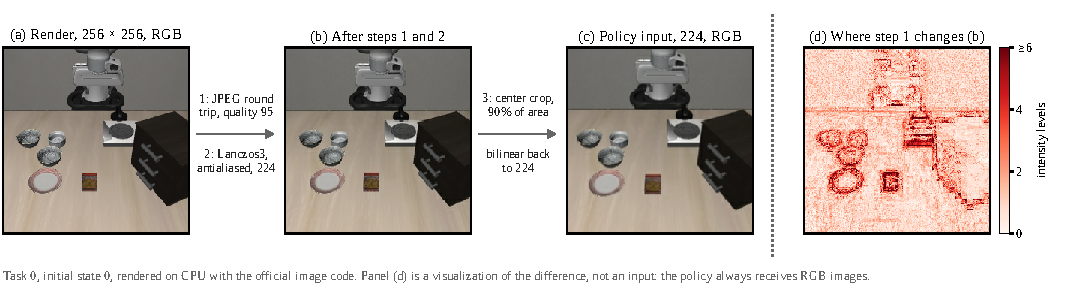
\includegraphics[width=\textwidth]{figures/pipeline.pdf}
\caption{The image steps of the official OpenVLA evaluation on LIBERO. (a) The RGB frame rendered by MuJoCo, after the \RotationDeg-degree rotation. (b) After step one, a JPEG encode and decode at quality \JpegQuality, and step two, a Lanczos3 resize to \InputRes{} with antialiasing. (c) The policy input after step three, a center crop of \CropAreaPct\% of the area resized back to \InputRes; the policy receives this RGB image. (d) A heat map of where step one changes image (b): for every pixel, the absolute change averaged over the R, G and B channels, in intensity levels. It visualizes the difference and is not an image any policy sees. The change sits on object edges, in $\DctBlock \times \DctBlock$ blocks, and its mean over the image is \FrameMeanDiff{} levels.}
\label{fig:pipeline}
\end{figure}

\subsection{The evaluation image pipeline}
\label{sec:pipeline}

We take the pipeline of the official OpenVLA evaluation on LIBERO as the reference (Figure~\ref{fig:pipeline}), as implemented in its code~\citep{openvlacode}. MuJoCo~\citep{mujoco} renders the third-person camera of the robosuite~\citep{robosuite} scene as a $\RenderRes \times \RenderRes$ RGB image, which is rotated by \RotationDeg{} degrees to match the training data. Step one encodes the image as JPEG with TensorFlow's default quality of \JpegQuality{} and decodes it immediately; a comment in the code states that this repeats the encoding of the dataset builder. Step two resizes the image to $\InputRes \times \InputRes$ with a Lanczos3 kernel~\citep{duchon1979} and antialiasing; the code comment states that this follows the resizing scheme of the Octo data loader~\citep{octo}, which OpenVLA uses for training. Step three keeps the central \CropAreaPct\% of the image area (each side scaled by \SideCrop) and resizes it back to \InputRes{} with bilinear interpolation; the evaluation code labels this crop as the counterpart of random-crop augmentation during training and asserts it for checkpoints trained with image augmentation. The environment is also seeded with a fixed value. OpenVLA-OFT~\citep{oft} applies the same steps to its third-person and wrist cameras~\citep{oftcode}. Every step keeps the three color channels.

Two properties explain why these steps may matter. JPEG~\citep{wallace1992} transforms each $\DctBlock \times \DctBlock$ block with the discrete cosine transform and quantizes the coefficients, high frequencies most coarsely, so its error concentrates in blocks that contain edges, which is where the outlines of the objects lie (Figure~\ref{fig:pipeline}d). Resizing changes the sampling grid: a kernel that is not low-pass enough lets high frequencies alias into the smaller image, and convolutional networks respond to such sampling details~\citep{azulay2019,zhang2019}. Lanczos and bilinear kernels filter differently, so the kernel can change the image a model sees.

\subsection{Variants}
\label{sec:variants}

Each variant changes one step and applies to every image the policy receives:
\begin{enumerate}
\item \emph{JPEG off}: the same TensorFlow resize call without the JPEG round trip;
\item \emph{Crop step off}: the evaluation script's own switch that skips step three. The policy then sees the full frame: objects appear about \Zoom\% smaller than in the center crop that matches training, and a band of about \Border{} pixels returns on each side;
\item \emph{Bilinear resize}: step two with the bilinear kernel, JPEG round trip and antialiasing unchanged;
\item \emph{Render at \InputRes}: the scene is rendered at $\InputRes \times \InputRes$, so step two no longer downsamples. The JPEG round trip and the Lanczos filter, now at scale one, are kept, so only the resolution changes. For OpenVLA-OFT this matches the official script, whose observation function applies the JPEG round trip and the resize to every frame before the model's own image preparation, which skips a second resize when an image is already at \InputRes~\citep{oftcode}; the harness logs the JPEG change of the first input in this cell (\OftRendMadMin{} to \OftRendMadMax{} intensity levels), which confirms that the round trip was applied.
\end{enumerate}
A fifth cell, the \emph{rerun}, repeats the reference unchanged. Before the variant cells ran, a check confirmed that the rewritten resize reproduces the official step pixel for pixel, so a variant differs from the reference in its one step only.

\subsection{Design choices}
\label{sec:design}

\emph{One step at a time.} Changing several steps together, as in earlier reproduction work~\citep{vlaevalrepo}, shows that the pipeline matters but not which step. Changing one step and keeping the rest attributes an effect to a step.

\emph{Paired episodes and a rerun.} LIBERO stores \NStates{} initial states per task, so a variant can be run from the same \NPairs{} states as the reference. Pairing removes the difference in difficulty between initial states from the comparison: only flips carry information, and the paired interval is narrower than an unpaired one (Appendix~\ref{app:ablation}). The rerun, an A/A comparison of the reference pipeline with itself, measures how many episodes change outcome when nothing changes on our stack.

\emph{Two policies with different action heads.} OpenVLA-7B picks each action dimension among \Bins{} discrete bins and acts one step per query; OpenVLA-OFT regresses continuous actions and executes chunks of \Chunk{} actions per query. Both start from the same vision backbone, so a difference in sensitivity between them may point to the action head and the decoding; the models also differ in their inputs (OpenVLA-OFT adds a wrist camera and the robot state) and in their fine-tuning, so this is a lead, not an attribution.

\emph{Color inputs.} The policies always receive RGB images, and we measure the size of an image change as the mean absolute difference over all pixels and the three color channels, on the scale of each channel; we call its unit an \emph{intensity level}. Appendix~\ref{app:eda} explains why grayscale inputs are not studied.

\subsection{Metrics and statistics fixed in advance}
\label{sec:stats}

The metric is the task success rate, reported with a Wilson \AlphaPct\% interval~\citep{wilson1927}. Each comparison with the reference reports the paired change in percentage points with a percentile bootstrap interval~\citep{efron1979} from \BootDraws{} resamples of the paired episodes, the counts $L$ and $G$, and the exact McNemar test~\citep{mcnemar1947}, which uses only the flips. These are standard paired statistics for policy comparisons~\citep{li2026paraphrase}; following recommendations for evaluations with few runs~\citep{agarwal2021,kressgazit2024}, we report intervals and do not read a non-significant result as the absence of an effect.

Before any variant was run we fixed one primary comparison: JPEG off against the reference for OpenVLA-7B, with \ThresholdPts{} points as the smallest loss that matters, about the size of the crop effect measured by vla-eval~\citep{vlaeval} and of many gaps between published models. The other \NSecondary{} comparisons form a secondary family with Holm correction~\citep{holm1979}. Because the power of the McNemar test depends on the share of flips, which was unknown, we also fixed a rule on \RuleDate{} \Year, before a pilot on initial states \SplitA: if at most \DiscThreshold\% of the pilot pairs flip, \NPairs{} pairs give \PowerTarget\% power to detect \ThresholdPts{} points and the test is run as planned; otherwise the primary result is the one-sided \AlphaPct\% upper bound on the loss, reported with its estimate and interval. The threshold comes from the exact power of the McNemar test for \NPairs{} pairs and a \ThresholdPts-point effect, computed over the binomial distribution of the number of flips (the script is released). The plan was written before the variant cells ran, but it was not committed to a public repository at the time, so its timing rests on our record; the dates that readers can check are those in the run metadata of every cell (Appendix~\ref{app:runlog}).

\subsection{How far flips alone move a score}
\label{sec:band}

The rule rests on the following calculation, which also gives the band used in the results. Suppose a change has no systematic effect, so each of the $f$ flips is independently equally likely to be a gain or a loss. Then the net change $D = G - L$ satisfies
\begin{equation}
G \sim \mathrm{Binomial}\!\left(f, \tfrac{1}{2}\right), \qquad D = 2G - f, \qquad \mathbb{E}[D] = 0, \qquad \mathrm{Var}[D] = 4 f \times \tfrac{1}{2} \times \tfrac{1}{2} = f,
\end{equation}
and with the normal approximation \AlphaPct\% of such changes fall within
\begin{equation}
D \in \pm 1.96\sqrt{f} \text{ episodes, that is, } \hat{\Delta} \in \pm \frac{1.96\sqrt{f}}{n}.
\label{eq:band}
\end{equation}
In the pilot, \PilotFlips{} of \PilotPairs{} OpenVLA-7B pairs flipped with JPEG off (\PilotDisc\%), which projects to $f \approx \PilotF$ at $n = \NPairs$, a standard deviation of \PilotSD{} episodes and a band of $\pm$\PilotBandEp{} episodes, or $\pm$\PilotBandPts{} points. A \ThresholdPts-point loss is only \ThresholdEp{} episodes of net change, inside the band, so \NPairs{} pairs give \PowerPilot\% power for it and about \PairsForEighty{} pairs would be needed for \PowerTarget\%. Because the pilot share of \PilotDisc\% exceeded \DiscThreshold\%, the rule selected the upper bound. More pairs were not an option: LIBERO-Spatial has \NPairs{} initial states, and on our stack, where an identical rerun changes almost no outcome (Section~\ref{sec:repro}), repeating a state adds almost no information. In the final runs the same comparison flipped $f = \SevJpegFlips$ episodes, which gives $\pm$\FinalBandEp{} episodes, or $\pm$\SevJpegBand{} points. Equation~\eqref{eq:band} is conditional on the observed $f$ and assumes no systematic effect; it describes how large a gap between two pipelines can be without being evidence that they differ.

\subsection{Open-loop action check}
\label{sec:olmethod}

Closed-loop success mixes the effect of a step with the chaos of the rollout. To see what a step does to the policy itself, we also give each policy identical observations through every pipeline and compare the predicted action with that of the reference pipeline, executing only the reference action. The observations are the first frame of each of the \NPairs{} initial states, and frames along the reference rollouts: every \OlStride{} query of OpenVLA-7B on the first \OlSevStates{} initial states of every task, and every query of OpenVLA-OFT on the first \OlOftStates. The frame for rendering at \InputRes{} comes from a second simulator instance that receives the same actions and the same random draw for the fixture placement. Both models are compared in one unit, the action bin of OpenVLA-7B: every action dimension is scaled to $[-1, 1]$ by the \PctLo{} and \PctHi{} percentiles of the training actions and split into \Bins{} bins, so a token difference of OpenVLA-7B is a difference in bins, and the continuous OpenVLA-OFT action is converted to the same scale and averaged over its chunk. We report the \SevTokenDims{} arm dimensions and, for OpenVLA-7B, the margin between the two highest logits of each action token. The check is exploratory: its summaries were chosen after the closed-loop results were known.

\section{Experimental Setup}
\label{sec:setup}

\paragraph{The suite.} LIBERO-Spatial~\citep{libero} has \NTasks{} tasks. Every task asks the robot to pick up a black bowl and place it on a plate, and the tasks differ only in where the target bowl is (between the plate and the ramekin, on the cookie box, in the top drawer of the wooden cabinet, on the stove, and so on), so the policy has to ground a spatial relation in the image while a second black bowl stands elsewhere on the table. On this suite the instruction is largely redundant with the scene: OpenVLA-OFT still succeeds in \ExtXieInstrLo\% to \ExtXieInstrHi\% of episodes when the instruction is made unreadable~\citep{xie2026language}, so the image carries most of the task information, which is one reason the image steps may matter here more than on suites where the instruction disambiguates the goal. Each task has a fixed file of \NStates{} initial states for evaluation, which gives \NPairs{} episodes per cell. An episode starts with \SettleSteps{} settle steps in which the robot holds still and runs for at most \PolicySteps{} policy steps; it succeeds when the goal predicate of the task holds.

\paragraph{Checkpoints.} We evaluate the released checkpoints unchanged; no model is trained or fine-tuned in this study. OpenVLA-7B was fine-tuned on LIBERO-Spatial with low-rank adaptation (rank \ExtOpenvlaLoraRank), on demonstrations re-rendered at $\RenderRes \times \RenderRes$, rotated by \RotationDeg{} degrees, with no-op actions and the failed demonstrations (\ExtOpenvlaDemosDropped{} of \ExtOpenvlaDemos) removed, using only the third-person camera, and with random-crop augmentation~\citep{openvla,openvlacode}; its authors report \ExtOpenvlaSpatial\% $\pm$ \ExtOpenvlaSpatialSe\% (mean and standard error over \ExtOpenvlaSeeds{} seeds of \NPairs{} episodes). OpenVLA-OFT was fine-tuned from OpenVLA per suite with low-rank adaptation for \ExtOftStepsLo{} to \ExtOftStepsHi{} gradient steps, with parallel decoding, chunks of \Chunk{} actions and an L1 regression loss, and receives the third-person image, a wrist-camera image and the robot state; its authors report \ExtOftSpatial\% on LIBERO-Spatial~\citep{oft}.

\paragraph{Cells and stack.} The study has \NCells{} cells: for each model, the reference, the rerun and \NVariants{} variants, all run between \FirstRunDate{} and \LastRunDate{} \Year{} on one \GpuName{} GPU per cell, with MuJoCo \MujocoVersion{} and greedy decoding for OpenVLA-7B. Appendix~\ref{app:runlog} lists the cells with their dates and host CPUs and the full software stack. The reference cells ran with the original evaluation scripts; the other cells ran with a thin harness that calls the original scripts and replaces only the image function of the step being changed. The host CPU, which can change LIBERO trajectories on its own~\citep{jiang2026bench}, was \CpuMain{} for every harness cell except two: OpenVLA-OFT with the crop step off ran on an \CpuOftCrop{} and OpenVLA-7B rendered at \InputRes{} on an \CpuSevRend; the original scripts do not record the CPU of the reference cells. The OpenVLA-OFT crop-off cell is thus the only OpenVLA-OFT cell whose host CPU is known to differ from the others; a rerun of it on an \CpuMain{} host repeats its outcomes (Appendix~\ref{app:cpucontrol}).
The harness logs one record per episode: task, initial state, outcome, number of steps, wall time, the placement of the cabinet and stove fixtures, hashes of the first frames and the size of the JPEG change on the first input. These records, with the log of the original script for the OpenVLA-OFT reference cell, are the data of every closed-loop table and figure. A pilot on initial states \SplitA, with \PilotCells{} cells of \PilotPairs{} episodes, ran on \PilotDate{} and served only the decision rule of Section~\ref{sec:stats} and the reproducibility check below; it is not pooled with the full cells. The open-loop check ran on \OlDates{} \Year{} on one GPU of the same type.

\paragraph{Same scene in every pair.} Pairing by initial state requires that the paired episodes start from the same scene, and a matching hash of the stored initial state is not enough: LIBERO restores the objects from the stored state but places some fixtures from the environment's own random draw, which depends on the environment's history, so the same stored state can yield different cabinet and stove positions~\citep{issue342}. Before each episode the harness checks the hash of the initial state against the benchmark file, and the hashes match in all pairs of every cell. Beyond that, in all \SceneCells{} harness cells the fixture placement agrees with the other cells of the same model in every pair, and so do the hashes of the first frames, except in the cells rendered at \InputRes, whose frames differ by design while their fixtures agree. All OpenVLA-7B harness cells use environment seed \EnvSeed, and all OpenVLA-OFT cells split the initial states into the same two runs (\SplitA{} and \SplitB) as its reference cell, so every environment goes through the same sequence of resets. The two reference cells ran with the original scripts, which log no fixtures, so for them the match of scenes rests on the reruns, which repeat \SevRerunSame{} and \OftRerunSame{} of \NPairs{} outcomes (Section~\ref{sec:repro}).

\paragraph{Shared runs.} Four cells of this study, the crop-step-off cells and the reference cells of OpenVLA-7B and OpenVLA-OFT on LIBERO-Spatial (\NPairs{} episodes each), are also used in a separate study by the same author, which addresses a different question. That study does not report the results of these cells and refers to this paper for them. No other run, analysis, figure, table or text of this paper appears in that study, and the two studies share only the evaluation harness.

\section{Results}
\label{sec:results}

\subsection{The reference runs reproduce published results}
\label{sec:repro}

With the official pipeline, OpenVLA-7B succeeds on \SevRefK/\NPairs{} episodes (\SevRefPct\%, Wilson \AlphaPct\% interval [\SevRefLo, \SevRefHi]), which contains the published \ExtOpenvlaSpatial\%. OpenVLA-OFT succeeds on \OftRefK/\NPairs{} (\OftRefPct\%, [\OftRefLo, \OftRefHi]), \OftRefVsPub{} points above the published \ExtOftSpatial\%.

On our stack the evaluation is close to deterministic. The OpenVLA-OFT rerun on \OftRerunDate{} repeats all \NPairs{} outcomes of the reference cell run on \OftRefDates. The OpenVLA-7B rerun, on another machine of the same type \RerunGapDays{} days after the reference, repeats \SevRerunSame{} of \NPairs{} outcomes, and \RerunSameStep{} of the \RerunBoth{} episodes that succeed in both end at exactly the same step. The full cells also repeat the pilot cells of \PilotDate{}: on initial states \SplitA, at most \PilotMaxDiffVsFinal{} of \PilotPairs{} outcomes differs in any of the cells that both runs contain. This floor belongs to our stack and policies and does not transfer. Two runs of one OpenVLA-OFT configuration differed on \ExtLiRerunPct\% of episodes in another stack~\citep{li2026paraphrase}; the LIBERO-CTRL repository reports \ExtCtrlOftSame{} of \NPairs{} OpenVLA-OFT episodes changing on the same GPU but \ExtCtrlUnivlaOtherGpu{} of \NPairs{} for UniVLA on another GPU~\citep{liberoctrlrepo}; and changing only the CPU, with the GPU type fixed, made the simulator state of OpenVLA-OFT diverge in \ExtJiangCpuTasks{} of \NTasks{} LIBERO tasks, \ExtJiangCpuPixelTasks{} of them up to pixels and actions~\citep{jiang2026bench}. An A/A floor has to be measured on the hardware and with the policy being compared. Against our floor of \OftRerunFlips{} to \SevRerunFlips{} flips in \NPairs, all but a few of the flips in a variant cell are caused by the variant.

% Generated by scripts/make_assets.py from the output of scripts/paired_stats.py of the results repository.
\begin{table*}[t]
\caption{Results on LIBERO-Spatial, 500 paired episodes per cell. Change: variant minus reference, in percentage points, with a 95\% percentile bootstrap interval over the paired episodes, computed exactly (no random draws). Lost: episodes that succeed under the reference and fail under the variant; gained: the reverse. $p$: exact two-sided McNemar test; Holm: adjusted over the seven secondary comparisons (the primary comparison, JPEG off for OpenVLA-7B, is not adjusted). Bound: one-sided 95\% upper bound on the loss, in points. Band: the 95\% range of the change that the observed number of flips $f$ leaves with no systematic effect, $\pm 1.96\sqrt{f}/500$ (Section~\ref{sec:band}).}
\label{tab:results}
\centering
\footnotesize
\setlength{\tabcolsep}{3.6pt}
\begin{tabular}{@{}llrccrrrrrrr@{}}
\toprule
Model & Cell & Successes & Rate (\%) [Wilson 95\%] & Change & Paired 95\% interval & Lost & Gained & $p$ & Holm & Bound & Band \\
\midrule
OpenVLA-7B & Reference & 425 & 85.0 [81.6, 87.9] & \multicolumn{8}{c}{reference cell} \\
 & Rerun (A/A) & 424 & 84.8 [81.4, 87.7] & $-$0.2 & [$-$1.0, +0.4] & 2 & 1 & 1.00 & - & 0.8 & $\pm$0.7 \\
 & JPEG off & 421 & 84.2 [80.7, 87.1] & $-$0.8 & [$-$4.2, +2.6] & 39 & 35 & 0.73 & - & 3.6 & $\pm$3.4 \\
 & Crop step off & 420 & 84.0 [80.5, 87.0] & $-$1.0 & [$-$4.6, +2.6] & 43 & 38 & 0.66 & 1.00 & 4.0 & $\pm$3.5 \\
 & Bilinear resize & 414 & 82.8 [79.2, 85.9] & $-$2.2 & [$-$5.8, +1.4] & 47 & 36 & 0.27 & 1.00 & 5.2 & $\pm$3.6 \\
 & Render at 224 & 427 & 85.4 [82.0, 88.2] & +0.4 & [$-$3.4, +4.2] & 45 & 47 & 0.92 & 1.00 & 2.8 & $\pm$3.8 \\
\midrule
OpenVLA-OFT & Reference & 495 & 99.0 [97.7, 99.6] & \multicolumn{8}{c}{reference cell} \\
 & Rerun (A/A) & 495 & 99.0 [97.7, 99.6] & 0.0 & [0.0, 0.0] & 0 & 0 & 1.00 & - & 0.0 & $\pm$0.0 \\
 & JPEG off & 491 & 98.2 [96.6, 99.1] & $-$0.8 & [$-$2.0, +0.4] & 7 & 3 & 0.34 & 1.00 & 1.8 & $\pm$1.2 \\
 & Crop step off & 483 & 96.6 [94.6, 97.9] & $-$2.4 & [$-$4.2, $-$0.8] & 15 & 3 & 0.008 & 0.053 & 3.8 & $\pm$1.7 \\
 & Bilinear resize & 496 & 99.2 [98.0, 99.7] & +0.2 & [$-$0.8, +1.2] & 3 & 4 & 1.00 & 1.00 & 0.6 & $\pm$1.0 \\
 & Render at 224 & 491 & 98.2 [96.6, 99.1] & $-$0.8 & [$-$2.0, +0.4] & 7 & 3 & 0.34 & 1.00 & 1.8 & $\pm$1.2 \\
\bottomrule
\end{tabular}
\end{table*}


\subsection{Effects of the image steps}
\label{sec:effects}

Table~\ref{tab:results} gives every cell. \emph{Primary result.} Turning the JPEG round trip off changes OpenVLA-7B by \SevJpegDiff{} points (\AlphaPct\% interval [\SevJpegLo, \SevJpegHi], \SevJpegLost{} episodes lost and \SevJpegGained{} gained, $p = \SevJpegP$). The one-sided \AlphaPct\% upper bound on the loss is \SevJpegUB{} points. It is above the \ThresholdPts{} points fixed in advance, so the study does not show that the JPEG step can be skipped: a loss of \ThresholdPts{} points remains possible, and a loss of more than \SevJpegUB{} points is unlikely.

\emph{Secondary results.} None of the \NSecondary{} secondary comparisons is significant after Holm correction. The closest is the crop step on OpenVLA-OFT: \OftCropDiff{} points ([\OftCropLo, \OftCropHi]), \OftCropLost{} lost and \OftCropGained{} gained, $p = \OftCropP$ before and \OftCropHolm{} after correction. It rests on two conditions that keep it exploratory. First, one task carries it: of the \OftCropLost{} lost episodes, \OftCropTaskFiveLost{} are in task \TaskFive{} (black bowl on the ramekin), where the crop-off cell succeeds in \OftTaskFiveCrop{} of \NStates{} episodes against \OftTaskFiveOthersMin{} to \OftTaskFiveOthersMax{} for every other OpenVLA-OFT pipeline; this is also the task that failed under MuJoCo \MujocoNewVersion{} (Section~\ref{sec:intro}), and without it the cell loses \OftCropNoFiveLost{} and gains \OftCropNoFiveGained{} episodes ($p = \OftCropNoFiveP$). Second, the cell ran on a different host CPU from every other OpenVLA-OFT harness cell (Section~\ref{sec:setup}), and a CPU change alone can change LIBERO trajectories of this policy~\citep{jiang2026bench}. % CPU-CONTROL: under rule (a) replace this second condition by "A rerun on the CPU of the other cells repeats its outcomes (Appendix~\ref{app:cpucontrol})"; under rule (b) report both runs here and state that the result depends on the CPU.
For OpenVLA-7B, turning the crop off changes success by \SevCropDiff{} points (bound on the loss \SevCropUB), consistent with the loss of about \ExtVeCropPts{} points that vla-eval reports for the crop over four suites~\citep{vlaeval}, but also with no loss. The bilinear kernel changes OpenVLA-7B by \SevBilDiff{} points (bound \SevBilUB) and rendering at \InputRes{} by \SevRendDiff. For OpenVLA-OFT the remaining changes lie between \OftJpegDiff{} and \OftBilDiff{} points. Appendix~\ref{app:ablation} checks these readings against the choices of the analysis.

\begin{figure}[t]
\centering
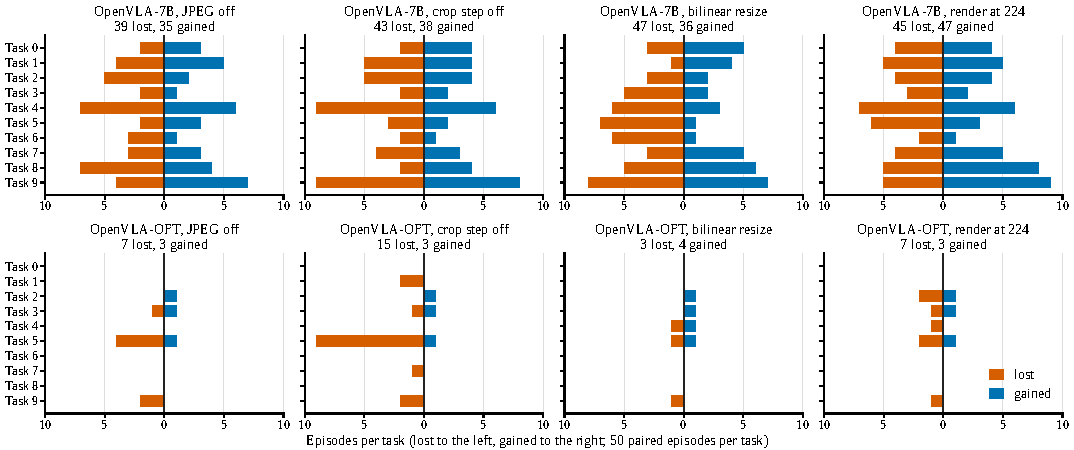
\includegraphics[width=\textwidth]{figures/flips.pdf}
\caption{Episodes that change outcome against the reference, per task, for every variant (\NStates{} paired episodes per task). Bars to the left count episodes lost by the variant, bars to the right episodes gained. The reruns change \SevRerunFlips{} OpenVLA-7B episodes and \OftRerunFlips{} OpenVLA-OFT episodes.}
\label{fig:flips}
\end{figure}

\subsection{Episodes that change outcome}
\label{sec:flips}

The net changes hide most of what happens (Figure~\ref{fig:flips}). Every OpenVLA-7B variant changes the outcome of \SevFlipsMin{} to \SevFlipsMax{} of the \NPairs{} episodes (\SevFlipPctMin\% to \SevFlipPctMax\%), in both directions and in all \NTasks{} tasks, against \SevRerunFlips{} for the rerun. The JPEG round trip alone, a change of about \EdaJpeg{} intensity levels to the policy input, flips \SevJpegFlips{} episodes. OpenVLA-OFT flips \OftFlipsMin{} to \OftFlipsMax{} episodes; with the crop or the JPEG step off, about half of them are in task \TaskFive. LIBERO-CTRL found the same cancellation for compound perturbations~\citep{liberoctrl}; here it appears for single, mild steps of the evaluator on clean frames.

The flips come from a common pool of fragile episodes rather than from one step. Over the five OpenVLA-7B pipelines (reference and four variants), \SevAlways{} episodes always succeed, \SevNever{} always fail and \SevChange{} (\SevChangePct\%) succeed under some pipelines only; \SevRescued{} of the \SevRefFail{} reference failures succeed under at least one variant. Any two variants share flipped episodes \SevOverlapRatioMin{} to \SevOverlapRatioMax{} times as often as expected by chance (\SevOverlapMin{} to \SevOverlapMax{} shared flips against \SevChanceMin{} to \SevChanceMax{} expected if flips were independent). For OpenVLA-OFT the counts are \OftAlways, \OftNever{} and \OftChange, with \OftChangeTaskFive{} of the \OftChange{} in task \TaskFive.

The trajectories change even when the outcome does not. Among OpenVLA-7B episodes that succeed under both the reference and a variant, only \SevSameStepMin\% to \SevSameStepMax\% end at the same step (median difference \SevStepDiffMin{} to \SevStepDiffMax{} steps), while the rerun ends at the same step in \RerunSameStep{} of \RerunBoth. For OpenVLA-OFT, compared with the rerun because the original script logs no step count, \OftSameStepMin\% to \OftSameStepMax\% end at the same step (median difference \OftStepDiffMin{} to \OftStepDiffMax). Because flip rates depend on the success level (\SevRefPct\% against \OftRefPct\%), these step differences are the fairer comparison of the two models: an image step changes almost every OpenVLA-7B trajectory and most OpenVLA-OFT trajectories, the latter by fewer steps.

\subsection{Open-loop action check}
\label{sec:openloop}

% Generated by scripts/make_assets.py from data/open_loop (scripts/open_loop_actions.py).
\begin{table}[t]
\caption{Open-loop action check: the same observation is given to the policy through each pipeline and the predicted action is compared with that of the reference pipeline. Each cell: share of observations whose arm action changes / mean absolute change of the six arm dimensions over all observations, in bins. OpenVLA-7B: difference in token index (a token spans 1/255 of the range between the 1st and 99th percentile of the training actions); any changed arm token counts. OpenVLA-OFT: absolute change averaged over the 8 actions of the chunk, in units of 1/256 of that range; a change above half a unit in any arm dimension counts. The two models' summaries are not directly comparable. First: the first observation of every initial state; along: observations along the reference rollout.}
\label{tab:openloop}
\centering
\footnotesize
\setlength{\tabcolsep}{2.5pt}
\begin{tabular}{@{}lcccc@{}}
\toprule
 & \multicolumn{2}{c}{OpenVLA-7B} & \multicolumn{2}{c}{OpenVLA-OFT} \\
\cmidrule(lr){2-3}\cmidrule(l){4-5}
Pipeline & First & Along & First & Along \\
Observations & 500 & 1713 & 500 & 1326 \\
\midrule
Same input again & 0\% / 0.0 & 0\% / 0.0 & 0\% / 0.0 & 0\% / 0.0 \\
JPEG off & 29\% / 3.3 & 35\% / 4.1 & 99\% / 0.9 & 84\% / 0.5 \\
Crop step off & 95\% / 14.4 & 91\% / 14.0 & 100\% / 10.1 & 100\% / 5.6 \\
Bilinear resize & 54\% / 6.9 & 55\% / 7.0 & 100\% / 2.4 & 97\% / 0.9 \\
Render at 224 & 78\% / 11.8 & 66\% / 8.6 & 100\% / 1.3 & 97\% / 0.8 \\
\bottomrule
\end{tabular}
\end{table}


Table~\ref{tab:openloop} gives the exploratory open-loop check of Section~\ref{sec:olmethod}. The reference rollouts used for it repeat the closed-loop cells (outcome and final step) in \OlSevTrajRepro{} of \OlSevTrajReproN{} OpenVLA-7B and \OlOftTrajRepro{} of \OlOftTrajReproN{} OpenVLA-OFT episodes, querying the same input twice never changes the action, and the frame rendered at \InputRes{} shows the same fixture placement as the reference frame in every observation, so the changes in the table are caused by the steps.

\emph{Every step changes the output.} On first frames, turning JPEG off changes at least one arm token of OpenVLA-7B in \OlSevFirstJpegChanged\% of the initial states, the bilinear kernel in \OlSevFirstBilChanged\%, rendering at \InputRes{} in \OlSevFirstRendChanged\% and the crop step in \OlSevFirstCropChanged\%; along the rollouts the order is the same. OpenVLA-OFT, whose output is continuous, moves on \OlOftTrajJpegChanged\% to all of the observations, but by little: on first frames \OlOftFirstJpegMean, \OlOftFirstBilMean{} and \OlOftFirstRendMean{} bins on average for JPEG off, bilinear and rendering at \InputRes, against \OlSevFirstJpegMean, \OlSevFirstBilMean{} and \OlSevFirstRendMean{} for OpenVLA-7B, and \OlOftTrajJpegMean{} to \OlOftTrajBilMean{} bins along the rollouts. The crop step is the exception: it moves OpenVLA-OFT by \OlOftFirstCropMean{} bins on first frames, close to the \OlSevFirstCropMean{} of OpenVLA-7B, and it is also the only step with a candidate closed-loop effect on OpenVLA-OFT. For both models the order of the steps differs from the order of their pixel changes (Appendix~\ref{app:eda}): the bilinear kernel moves the pixels least but moves the action more than the JPEG round trip, so the mean pixel difference is a poor guide to what a step does to the policy.

\emph{Discrete jumps, not only near-ties.} OpenVLA-7B tokens whose reference choice is nearly tied (the two highest logits less than \MarginLow{} apart, \OlSevFirstMarginLowShare\% of the arm tokens on first frames) are changed by at least one of the four variants in \OlSevFirstMarginLow\% of cases, against \OlSevFirstMarginHigh\% for confident tokens (margin of \MarginHigh{} or more, \OlSevFirstMarginHighShare\%); along the rollouts the shares are \OlSevTrajMarginLow\% and \OlSevTrajMarginHigh\%. Near-ties make a token easier to switch, but confident tokens switch too, and a switched token jumps by many bins: on first frames the median largest change per observation is \OlSevFirstCropMedmax{} bins with the crop off and \OlSevFirstRendMedmax{} when rendering at \InputRes.

\emph{First actions and flips.} We find no association between a changed first action and a flip: with JPEG off, \OlSevFirstJpegFlipIfChanged\% of the episodes whose first OpenVLA-7B action changed flip in the closed loop, against \OlSevFirstJpegFlipIfSame\% of those whose first action did not change (\OlSevFirstJpegNChanged{} of the \NPairs{} first actions changed); for the bilinear kernel the two rates are \OlSevFirstBilFlipIfChanged\% and \OlSevFirstBilFlipIfSame\%. Whether an episode flips appears to be decided later in the rollout, as differences accumulate, which agrees with the almost universal change of the OpenVLA-7B success step (Section~\ref{sec:flips}).

\subsection{Comparison with other evaluations of the same checkpoints}
\label{sec:compare}

% Generated by scripts/make_assets.py; numbers of other studies come from data/external_numbers.json.
\begin{table}[t]
\caption{LIBERO-Spatial success of the same released checkpoints in other evaluations (numbers as reported) and in this study. OpenVLA: mean and standard error over three seeds of 500 episodes. vla-eval: its published per-episode results, which we pair with ours (Section~\ref{sec:compare}); its image steps and environment loop are its own. StableVLA: checkpoint identifiers, evaluation script and episode count not stated.}
\label{tab:compare}
\centering
\small
\begin{tabular}{@{}lcc@{}}
\toprule
Evaluation & OpenVLA-7B (\%) & OpenVLA-OFT (\%) \\
\midrule
OpenVLA paper, official code~\citep{openvla} & 84.7 $\pm$ 0.9 & - \\
OpenVLA-OFT paper, official code~\citep{oft} & - & 97.6 \\
vla-eval harness~\citep{vlaevalrepo} & 86.6 & - \\
StableVLA, clean images~\citep{stablevla} & 80.0 & 92.6 \\
\midrule
This study, reference cell & 85.0 [81.6, 87.9] & 99.0 [97.7, 99.6] \\
This study, four single-step variants & 82.8-85.4 & 96.6-99.2 \\
\bottomrule
\end{tabular}
\end{table}


\begin{figure}[t]
\centering
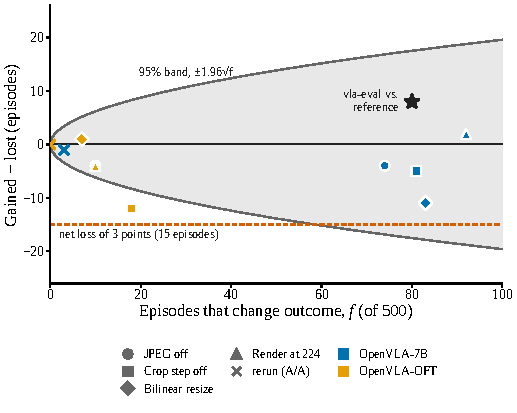
\includegraphics[width=0.55\textwidth]{figures/band.pdf}
\caption{Net change against the number of flips for every comparison with the reference. The shaded area is the \AlphaPct\% band of Equation~\eqref{eq:band}, the range of net changes that flips alone produce when a change has no systematic effect. Every comparison falls inside it except OpenVLA-OFT with the crop step off; the dashed line marks the \ThresholdPts-point loss fixed in advance.}
\label{fig:band}
\end{figure}

Table~\ref{tab:compare} sets our results beside other evaluations of the same released checkpoints. For OpenVLA-7B the published values range from \ExtStableClean\% to \ExtVeSpatial\%, our reference cell gives \SevRefPct\% and our four variants \SevVarMinPct\% to \SevVarMaxPct\%. The vla-eval harness publishes the outcome of every episode~\citep{vlaevalrepo}, which lets us compare it with our cells on the same \NPairs{} initial states. It succeeds on \VeK/\NPairs{} against our \SevRefK. Initial state by initial state, \VeOnlyTheirs{} succeed only in its run and \VeOnlyOurs{} only in ours: the two evaluations disagree on \VeFlips{} initial states while their totals differ by \VeGap{} points ($p = \VeP$), inside the band of $\pm$\VeBand{} points that \VeFlips{} flips leave. This is an illustration, not a controlled comparison. vla-eval implements the image steps itself: it encodes JPEG with Pillow at the library's default quality of \ExtVeJpegQuality~\citep{pillow} where the official code uses TensorFlow at \JpegQuality, resizes with Pillow's Lanczos filter, and takes the crop with sides rounded down to whole pixels and resizes it back with Lanczos where the official code uses bilinear interpolation~\citep{vlaevalrepo}. It also runs its own environment loop, and because LIBERO places some fixtures according to the environment's history~\citep{issue342}, the same initial state need not give the same scene in the two harnesses. And part of the disagreement may be vla-eval's own run-to-run variation, since two of its runs agree on only \ExtRoboscopeSelfLo\% to \ExtRoboscopeSelfHi\% of episodes on another suite~\citep{roboscope}.

Figure~\ref{fig:band} puts all comparisons on one scale. Every comparison except OpenVLA-OFT with the crop step off lies inside the band of Equation~\eqref{eq:band}; that one lies outside, in line with its candidate effect. With \SevFlipsMin{} to \SevFlipsMax{} flips, a change with no systematic effect moves a \NPairs-episode OpenVLA-7B score within about $\pm$\SevBandMin{} to $\pm$\SevBandMax{} points; for OpenVLA-OFT, with \OftFlipsMin{} to \OftFlipsMax{} flips, within $\pm$\OftBandMin{} to $\pm$\OftBandMax. Differences of that size between two evaluation pipelines are not evidence that the pipelines differ. The StableVLA value for OpenVLA-7B lies \StableGapPts{} points below our reference, more than flips alone produce in our paired comparisons; its episodes are not paired with ours and its evaluation details are not stated, so the cause of the gap is unknown.

\section{Discussion}
\label{sec:discussion}

\paragraph{Why can a change of about one intensity level flip an episode?} The open-loop check bears on three explanations. First, the closed loop amplifies small differences: we find no association between a changed first action and a flip, while almost every OpenVLA-7B trajectory ends at a different step, so flips appear to be decided by differences that accumulate over the rollout. Second, OpenVLA-7B chooses each action dimension greedily among \Bins{} bins: nearly tied tokens switch most often, but confident tokens switch as well and switched tokens jump by tens of bins, so a step moves OpenVLA-7B between distinct actions rather than nudging it. Third, OpenVLA-OFT regresses continuous actions: under the three mild steps it moves by \OlOftFirstJpegMean{} to \OlOftFirstBilMean{} bins on first frames and under one bin along the rollouts, and only the crop step, which moves it by about ten bins, shows a candidate loss in the closed loop. These observations fit the explanations without proving them.

\paragraph{What this means for practice.} Matching the image steps is cheap, and our bounds do not license skipping them. For the two checkpoints studied here, the larger risk to comparisons is not one step: any change to the evaluation reshuffles the fragile episodes, and other studies show that for some stacks even a different machine does~\citep{jiang2026bench,roboscope}. Score gaps within the band of Equation~\eqref{eq:band} should not be read as differences between models or pipelines unless the episodes are paired and the flips are reported. For policies that sample their actions the floor is higher still: the LIBERO-CTRL repository reports that \ExtCtrlSampledLo\% to \ExtCtrlSampledHi\% of rollouts of sampling policies change outcome from one rollout to the next~\citep{liberoctrlrepo}, so an A/A floor has to be measured on the policy being compared, not borrowed from a deterministic one.

We therefore recommend that evaluations (i) state their image pipeline and match the original one; (ii) compare pipelines or models on paired initial states, with the environment loop matched so that paired episodes start from the same scene, and report lost and gained episodes; (iii) measure an A/A floor on the same hardware and policy; and (iv) read a score gap within $\pm \Zval\sqrt{f}/n$ as no evidence of a difference.

\paragraph{Limitations.} The study covers one suite in simulation, one released checkpoint per model, one simulator version and one GPU type, so nothing is claimed about real robots, other suites or other policies. On LIBERO-Spatial the instruction is largely redundant with the image~\citep{xie2026language}, so the steps may matter less on suites where the instruction carries the goal, such as LIBERO-Goal. Closed-loop success is a coarse, noisy measure: a step triggers flips whose direction does not follow the step, so the study bounds the effect of a step rather than measuring it, and \NPairs{} initial states are not enough to resolve \ThresholdPts{} points at this rate of flips. OpenVLA-OFT is close to full success, which hides losses. The candidate effect of the crop on OpenVLA-OFT rests on one task; a rerun of its cell on the CPU of the other OpenVLA-OFT cells repeats its outcomes (Appendix~\ref{app:cpucontrol}). with the control rerun.
The image-level measurements of Appendix~\ref{app:eda} use frames rendered on a CPU; the GPU frames of the runs agree with them to within a few hundredths of a level. The open-loop check is exploratory: its summaries were chosen after the closed-loop results, it covers the first frame of every initial state but rollouts of only \OlSevStates{} (OpenVLA-7B) and \OlOftStates{} (OpenVLA-OFT) initial states per task, and it measures OpenVLA-OFT in the bins of OpenVLA-7B, averaged over a chunk.

\section{Conclusion}
\label{sec:conclusion}

We changed the image steps of the official OpenVLA evaluation one at a time and measured two released OpenVLA-family checkpoints on all \NPairs{} initial states of LIBERO-Spatial, with paired episodes, a rerun as the noise floor and a primary analysis fixed before any variant was run. No step has a net effect that \NPairs{} pairs can resolve: for the primary comparison, turning off the JPEG round trip, the loss is at most \SevJpegUB{} points with \AlphaPct\% confidence, which does not rule out the \ThresholdPts{} points that matter, and the closest secondary effect, the center crop on OpenVLA-OFT, is exploratory. Yet every step, including a JPEG change of about one intensity level, flips \SevFlipPctMin\% to \SevFlipPctMax\% of OpenVLA-7B episodes in both directions and changes almost every trajectory, so the cancellation that paired evaluations have reported for large perturbations already occurs for the evaluator's own steps on clean frames. The same paired design applies to other suites, to more checkpoints per model and to other evaluation choices, such as the simulator version.


\bibliography{refs}
\bibliographystyle{tmlr}

\appendix
\section{Run log and setup}
\label{app:runlog}

Table~\ref{tab:cells} lists the \NCells{} cells and the CPU control of Appendix~\ref{app:cpucontrol} with the date each one started and its host CPU, and Table~\ref{tab:setup} lists the software and hardware, read from the metadata that every cell records. In order: the reference cells ran on \RefDates; our record dates the decision rule to \RuleDate; the pilot ran on \PilotDate; the rerun and variant cells on \VariantDates; the open-loop check on \OlDates; and the CPU control on \CpuCtrlDates.

% Generated by scripts/make_assets.py from run_meta.json and the episode records of every cell.
\begin{table}[t]
\caption{The twelve cells of the study and their run log. Each cell runs the 500 (task, initial state) pairs of LIBERO-Spatial. Date: day of 2026 on which the cell started; hours: summed episode time on one GPU (not logged by the original OpenVLA-OFT script); host CPU as recorded in the run metadata (the two reference cells ran with the original scripts, which do not record it). Every cell ran on one NVIDIA RTX PRO 4500 Blackwell GPU.}
\label{tab:cells}
\centering
\scriptsize
\setlength{\tabcolsep}{3pt}
\begin{tabular}{@{}llL{0.36\columnwidth}lrl@{}}
\toprule
Model & Cell & What changes & Date & Hours & Host CPU \\
\midrule
OpenVLA-7B & Reference & original evaluation script, unchanged & 6 Oct & 5.2 & not logged \\
 & Rerun (A/A) & reference repeated unchanged & 28 Oct & 4.6 & EPYC 7663 \\
 & JPEG off & no JPEG round trip before the resize & 28 Oct & 4.5 & EPYC 7663 \\
 & Crop step off & no center crop (script flag) & 28 Oct & 4.6 & EPYC 7663 \\
 & Bilinear resize & bilinear instead of Lanczos3 resize & 29 Oct & 4.7 & EPYC 7663 \\
 & Render at 224 & cameras rendered at 224, not 256 & 29 Oct & 4.2 & EPYC 7443 \\
\midrule
OpenVLA-OFT & Reference & original evaluation script, unchanged & 3 Oct, 5 Oct & - & not logged \\
 & Rerun (A/A) & reference repeated unchanged & 29 Oct & 0.7 & EPYC 7663 \\
 & JPEG off & no JPEG round trip before the resize & 29 Oct & 0.7 & EPYC 7663 \\
 & Crop step off & no center crop (script flag) & 29 Oct & 0.7 & EPYC 7763 \\
 & Bilinear resize & bilinear instead of Lanczos3 resize & 29 Oct & 0.6 & EPYC 7663 \\
 & Render at 224 & cameras rendered at 224, not 256 & 29 Oct & 0.7 & EPYC 7663 \\
\bottomrule
\end{tabular}
\end{table}

% Generated by scripts/make_assets.py from run_meta.json of the cells.
\begin{table}[t]
\caption{Evaluation setup, read from the run metadata that every cell records.}
\label{tab:setup}
\centering
\footnotesize
\begin{tabular}{@{}L{0.22\columnwidth}L{0.71\columnwidth}@{}}
\toprule
Item & Value \\
\midrule
Checkpoints & \path{openvla/openvla-7b-finetuned-libero-spatial}; \path{moojink/openvla-7b-oft-finetuned-libero-spatial} \\
Episodes & LIBERO-Spatial, 10 tasks $\times$ 50 stored initial states = 500 per cell; 10 settle steps + at most 220 policy steps \\
Simulator & MuJoCo 3.3.7, robosuite 1.4.1, headless offscreen rendering (EGL) \\
Libraries & PyTorch 2.8.0, Transformers 4.40.1, TensorFlow 2.16.2, NumPy 1.26.4 \\
Model settings & seed 7, environment seed 0, scaled dot-product attention (SDPA), greedy decoding (OpenVLA-7B); chunks of 8 actions (OpenVLA-OFT) \\
Code & OpenVLA commit \texttt{c8f03f4}, OpenVLA-OFT commit \texttt{e4287e9}, LIBERO commit \texttt{8f1084e} \\
Hardware & one NVIDIA RTX PRO 4500 Blackwell (32 GB) per cell; host CPU per cell in Table~\ref{tab:cells} (EPYC 7663 for every harness cell except OpenVLA-OFT with the crop step off, EPYC 7763, and OpenVLA-7B rendered at 224, EPYC 7443) \\
Compute & 31 GPU hours for the 5,500 timed episodes of Table~\ref{tab:cells} (the original OpenVLA-OFT script does not log time) \\
\bottomrule
\end{tabular}
\end{table}


\subsection{Pilot cells}
\label{app:pilot}

Before the full variant cells, a pilot ran \PilotCells{} cells of \PilotPairs{} episodes on initial states \SplitA{} of every task, all on \PilotDate{} on one machine (Table~\ref{tab:pilot}): the reference, an identical rerun and JPEG off for both models, and the crop step off for OpenVLA-7B. Its JPEG-off comparison for OpenVLA-7B gave the share of flips, \PilotDisc\%, that the decision rule of Section~\ref{sec:stats} uses, and the pilot cells are compared with the full cells in the reproducibility check of Section~\ref{sec:repro}. The pilot is not pooled with the full cells, but its initial states are among theirs and the full cells repeat its outcomes, so \PilotPairs{} of the \NPairs{} pairs of the primary comparison were known before the full cells ran; Section~\ref{sec:effects} reports the other \OutPairs{} separately. The per-episode records and run metadata of the pilot cells are released with the paper source.

% Generated by scripts/make_assets.py from data/pilot_states_0-19/*/run_meta.json and episodes.jsonl.
\begin{table}[t]
\caption{The pilot cells, run before the full cells on initial states 0-19 of every task (200 episodes per cell). Start: day and time (clock of the cloud instance) at which the cell started, from its run metadata. Successes: of 200. Differ: outcomes that differ from the full cell of the same pipeline on the same 200 pairs. The pilot included two variant steps; it fixed the share of flips used by the decision rule and is not pooled with the full cells.}
\label{tab:pilot}
\centering
\footnotesize
\begin{tabular}{@{}llllrl@{}}
\toprule
Model & Cell & Start & Successes & Differ & Host CPU \\
\midrule
OpenVLA-7B & Reference & 12 Oct 02:20 & 161 & 0 & EPYC 7713P \\
 & Rerun (A/A) & 12 Oct 09:21 & 161 & 0 & EPYC 7713P \\
 & JPEG off & 12 Oct 04:26 & 168 & 0 & EPYC 7713P \\
 & Crop step off & 12 Oct 07:15 & 167 & 1 & EPYC 7713P \\
OpenVLA-OFT & Reference & 12 Oct 01:55 & 198 & 0 & EPYC 7713P \\
 & Rerun (A/A) & 12 Oct 06:52 & 198 & 0 & EPYC 7713P \\
 & JPEG off & 12 Oct 06:28 & 196 & 0 & EPYC 7713P \\
\bottomrule
\end{tabular}
\end{table}


\subsection{CPU control of the OpenVLA-OFT crop-off cell}
\label{app:cpucontrol}

The OpenVLA-OFT crop-off cell ran on an \CpuOftCrop{} host, while every other OpenVLA-OFT harness cell ran on an \CpuMain. We reran it on an \CpuCtrlCpu{} host, with the same split of initial states and the same configuration. The rerun succeeds on \CpuCtrlK{} of \NPairs{} episodes, and its outcome is the same as the original cell on \CpuCtrlSame{} of \NPairs{} initial states, which is the floor of the identical OpenVLA-OFT rerun on this stack. Against the reference cell it loses \CpuCtrlLost{} and gains \CpuCtrlGained{} episodes ($p = \CpuCtrlP$), as the original cell does. The host CPU therefore does not account for the result of the crop step on OpenVLA-OFT, and the original cell stays the reported result; the effect remains exploratory for the reasons given in Section~\ref{sec:effects}.\HookCpuAppendix{}

\subsection{Runs under MuJoCo \MujocoNewVersion}
\label{app:mujoco}

The motivating example of Section~\ref{sec:intro} comes from two reproduction runs made before this study: OpenVLA-7B on initial states \SplitA{} of every task under MuJoCo \MujocoNewVersion{} (\MujocoNewK{} of \PilotPairs, \MujocoNewPct\%, with \MujocoNewTaskFive{} of \PilotStates{} in task \TaskFive), and OpenVLA-OFT on task \TaskFive{} only (\OftNewTaskFive). Under MuJoCo \MujocoVersion{} the same \PilotPairs{} OpenVLA-7B episodes give \MujocoOldK{} (\MujocoOldPct\%), the outcomes of our reference cell on those states. Their per-task results and the OpenVLA-OFT log are released with the paper source; they record the checkpoint, the initial states and the GPU but not the full software stack, so the example shows how far an evaluation can move and is not a controlled comparison of simulator versions.

\section{Image-level measurements}
\label{app:eda}

\begin{figure}[t]
\centering
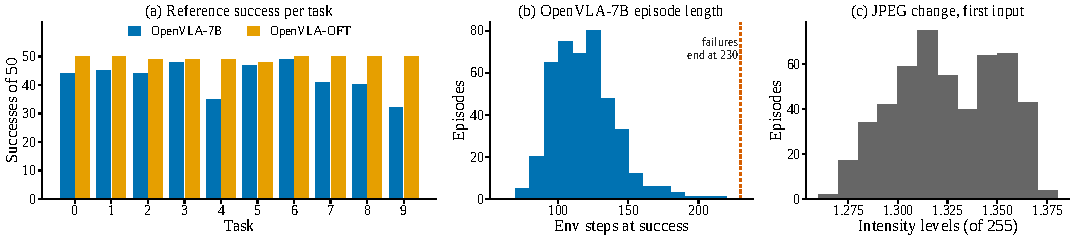
\includegraphics[width=\textwidth]{figures/data.pdf}
\caption{Data of the reference cells (\NPairs{} episodes per model). (a) Successes per task. (b) Number of environment steps at which successful OpenVLA-7B episodes end; failures always run to the limit of \MaxSteps{} (\SettleSteps{} settle steps plus \PolicySteps{} policy steps). (c) Mean absolute change that the JPEG round trip makes to the first resized image, before the crop, of each of the \NPairs{} OpenVLA-7B initial states, rendered on the GPU and logged by the JPEG-off cell, whose first frames equal those of every other harness cell.}
\label{fig:data}
\end{figure}

\paragraph{Outcomes.} Figure~\ref{fig:data}a shows the success of the reference cells per task. OpenVLA-7B ranges from \TaskMinSev{} to \TaskMaxSev{} of \NStates, with task \TaskNine{} (bowl on the wooden cabinet) and task \TaskFour{} (bowl in the top drawer) the hardest, while OpenVLA-OFT succeeds on \TaskMinOft{} to \TaskMaxOft{} in every task. Successful OpenVLA-7B episodes end after a median of \SuccStepMedian{} environment steps (interquartile range \SuccStepQone-\SuccStepQthree), well before the limit of \MaxSteps{} at which every failure ends (Figure~\ref{fig:data}b); whether a failed rollout would succeed later is unknown, but cutting the budget does not reduce the flips (Appendix~\ref{app:ablation}).

\paragraph{Size of the image changes.} On the GPU-rendered first frame of all \NPairs{} episodes, the JPEG round trip changes the resized image before the crop by \GpuMadMean{} intensity levels on average (range \GpuMadMin{} to \GpuMadMax, Figure~\ref{fig:data}c), and the bilinear kernel changes it by \GpuBilMean. The change is almost the same in every scene. To compare all steps on the final policy input, we rendered the first frame of the first \EdaStates{} initial states of every task on a CPU (\EdaFrames{} frames) and passed each through the official code with and without each change (Table~\ref{tab:eda}). On those frames the JPEG change before the crop is \CpuPreMean{} levels against \GpuSameMean{} for the same states on the GPU, so the CPU frames are representative. The bilinear kernel, the JPEG round trip and rendering at \InputRes{} change the policy input by \EdaBil, \EdaJpeg{} and \EdaRend{} levels on average; the JPEG change touches \EdaJpegChanged\% of the pixels. Turning the crop off is a different kind of change: it rescales and shifts the whole image, which gives a large per-pixel difference (\EdaCrop{} levels) although the content is the same. For scale, the mildest ImageNet-C JPEG corruption~\citep{imagenetc} changes the input by \EdaCone{} levels, and severity \ExtStableSevLo, which lowers OpenVLA from \ExtStableClean\% to \ExtStableJpegThree\% in StableVLA's evaluation~\citep{stablevla}, by \EdaCthree{} levels, \EdaCthreeRatio{} times the change of the JPEG step.

% Generated by scripts/make_assets.py from eda/frames.jsonl (scripts/eda_frames.py).
\begin{table}[t]
\caption{How far each change moves the $224 \times 224$ RGB policy input of OpenVLA-7B, against the input of the official pipeline. Mean: mean absolute difference over all pixels and the three color channels, in intensity levels (0-255), averaged over 50 first frames (initial states 0-4 of every task, rendered on CPU); range over frames; p99: 99th percentile of the per-value change; changed: share of pixels with any change. The four steps of this study are on top; the grayscale input and the ImageNet-C JPEG corruption are not part of any evaluation pipeline and are listed for scale.}
\label{tab:eda}
\centering
\footnotesize
\setlength{\tabcolsep}{3.5pt}
\begin{tabular}{@{}lrcrr@{}}
\toprule
Change & Mean & Range & p99 & Changed (\%) \\
\midrule
Bilinear resize & 0.64 & 0.59-0.70 & 8 & 40 \\
JPEG off & 1.26 & 1.21-1.30 & 6 & 96 \\
Render at 224 & 1.76 & 1.61-1.90 & 17 & 79 \\
Crop step off (rescales) & 8.33 & 7.74-8.96 & 102 & 88 \\
\midrule
Grayscale (luminance only) & 6.25 & 6.08-6.44 & 24 & 95 \\
ImageNet-C JPEG, sev.~1 (q.~25) & 3.44 & 3.31-3.59 & 18 & 99 \\
ImageNet-C JPEG, sev.~3 (q.~15) & 4.60 & 4.45-4.74 & 23 & 100 \\
ImageNet-C JPEG, sev.~5 (q.~7) & 7.65 & 7.49-7.86 & 32 & 100 \\
\bottomrule
\end{tabular}
\end{table}


\paragraph{Color inputs, and why no grayscale.} The policies always receive RGB images, in the reference and in every variant, and the intensity level is the average size of the change in the RGB values the policy receives, the same quantity as the mean absolute error used for image quality; it is not a grayscale conversion. We did not study grayscale inputs, for three reasons. Both checkpoints were trained on RGB frames, so a grayscale input would be a mismatch larger than any of the three steps that keep the geometry: replacing the policy input by its luminance changes it by \EdaGray{} intensity levels, about \EdaGrayRatio{} times the change of the JPEG round trip (Table~\ref{tab:eda}). Grayscale also removes the chroma that separates surfaces of similar brightness, and the policy has to find a particular black bowl among similar objects. And the question is which steps of the real evaluation pipeline must be matched, and grayscale is not one of them.

\section{Ablation of the analysis}
\label{app:ablation}

The variants themselves are an ablation of the evaluation pipeline: each removes or replaces one component and keeps the rest. Table~\ref{tab:ablation} ablates the choices of the analysis on the primary comparison and checks the reading of the secondary results.

% Generated by scripts/make_assets.py.
\begin{table}[t]
\caption{Ablation of the analysis choices on the primary comparison (JPEG off, OpenVLA-7B), and checks of the reading of the secondary results. Change and 95\% bootstrap interval in points; bound: one-sided 95\% upper bound on the loss.}
\label{tab:ablation}
\centering
\footnotesize
\setlength{\tabcolsep}{3pt}
\begin{tabular}{@{}L{0.45\columnwidth}L{0.49\columnwidth}@{}}
\toprule
Choice removed or changed & Result \\
\midrule
Paired bootstrap (as reported) & $-$0.8 [$-$4.2, +2.6], width 6.8, bound 3.6 \\
Pairing removed (cells treated as independent samples) & $-$0.8 [$-$5.2, +3.6], width 8.8, bound 4.6 \\
200 initial states (0-19) instead of 500 & +3.5 [$-$2.5, +9.5], width 12.0; 14 lost, 21 gained \\
One task left out (10 analyses) & change between $-$1.6 and $-$0.2 \\
Step budget cut from 230 to 180 / 150 / 120 env steps & flips 81 / 90 / 87 (against 74) \\
Initial states 20-49 only (outside the pilot) & $-$3.7 [$-$7.7, +0.3], bound 7.0; 25 lost, 14 gained, $p = 0.11$ \\
Tasks resampled instead of episodes & [$-$3.0, +1.6], bound 2.8 (OpenVLA-OFT crop off: [$-$5.8, 0.0]) \\
Logged rerun as the reference instead of the reference cell & $-$0.6 [$-$4.0, +2.8], bound 3.4; four variants: 75-93 flips, every $p \geq 0.33$ \\
\midrule
OpenVLA-OFT crop off without task 5 & 6 lost, 2 gained, $p = 0.29$ (with task 5: 15 lost, 3 gained) \\
Variant against variant instead of against the reference (OpenVLA-7B, 6 pairs) & 85-99 flips, every $p \geq 0.23$ \\
Reference cell split by initial state (OpenVLA-7B) & states 0-19: 161 vs 163-168; states 20-49: 264 vs 251-260 \\
\bottomrule
\end{tabular}
\end{table}


\emph{Pairing.} Treating the reference and the JPEG-off cell as independent samples widens the \AlphaPct\% interval from \AblPairedW{} to \AblUnpairedW{} points and raises the bound on the loss from \AblPairedUB{} to \AblUnpairedUB{} points. Neither interval resolves \ThresholdPts{} points.

\emph{Number of initial states.} With only initial states \SplitA, the size of the pilot, the same comparison reads \AblFirstDiff{} points with an interval \AblFirstW{} points wide; on states \SplitB{} it reads \OutDiff. A \PilotPairs-episode result would have suggested that turning JPEG off helps.

\emph{Unit of resampling.} Resampling the \NTasks{} tasks instead of the episodes gives [\ClusJpegLo, \ClusJpegHi] for the primary comparison and [\ClusOftCropLo, \ClusOftCropHi] for the OpenVLA-OFT crop. With only \NTasks{} clusters this interval is itself unreliable, and the reading fixed in advance uses the episode bootstrap; we report it because it puts zero inside the crop interval.

\emph{Rerun as the reference.} With the logged OpenVLA-7B rerun as the reference, whose harness records the CPU, the fixtures and the first frames, the four variants flip \VrFlipsMin{} to \VrFlipsMax{} episodes, change success by \VrDiffMin{} to \VrDiffMax{} points and are not significant ($p \geq \VrPMin$), as against the reference cell.

\emph{Single tasks and the step budget.} Leaving any one task out moves the primary estimate only between \AblLooMin{} and \AblLooMax{} points, so no single task drives it. Cutting the step budget from \MaxSteps{} to \BudgetA, \BudgetB{} or \BudgetC{} steps does not reduce the flips, so they are not successes that arrive just before the time limit. The OpenVLA-OFT crop result does depend on one task: without task \TaskFive{} it loses \OftCropNoFiveLost{} and gains \OftCropNoFiveGained{} episodes ($p = \OftCropNoFiveP$). Against the bilinear cell instead of the reference, the crop-off cell loses \OftCropVsBilLost{} and gains \OftCropVsBilGained{} ($p = \OftCropVsBilP$, uncorrected), the only candidate for a real effect in the study, and an exploratory one, for the two reasons given in Section~\ref{sec:effects}.

\emph{Choice of reference.} Comparing the OpenVLA-7B variants with each other instead of with the reference gives \SevVVfMin{} to \SevVVfMax{} flips per pair and no significant difference ($p \geq \SevVVpMin$). The reference cell is also slightly lucky: on states \SplitA{} every variant scores above it (\SevSplitVarAMin{} to \SevSplitVarAMax{} against \SevSplitRefA), and on states \SplitB{} every variant scores below it (\SevSplitVarBMin{} to \SevSplitVarBMax{} against \SevSplitRefB). The direction of a small net change can depend on which run is called the reference.

\section{Comparison with other evaluations}
\label{app:compare}

% Generated by scripts/make_assets.py; numbers of other studies come from data/external_numbers.json.
\begin{table}[t]
\caption{LIBERO-Spatial success of the same released checkpoints in other evaluations (numbers as reported) and in this study. OpenVLA: mean and standard error over three seeds of 500 episodes. vla-eval: its published per-episode results, which we pair with ours (Section~\ref{sec:compare}); its image steps and environment loop are its own. StableVLA: checkpoint identifiers, evaluation script and episode count not stated.}
\label{tab:compare}
\centering
\small
\begin{tabular}{@{}lcc@{}}
\toprule
Evaluation & OpenVLA-7B (\%) & OpenVLA-OFT (\%) \\
\midrule
OpenVLA paper, official code~\citep{openvla} & 84.7 $\pm$ 0.9 & - \\
OpenVLA-OFT paper, official code~\citep{oft} & - & 97.6 \\
vla-eval harness~\citep{vlaevalrepo} & 86.6 & - \\
StableVLA, clean images~\citep{stablevla} & 80.0 & 92.6 \\
\midrule
This study, reference cell & 85.0 [81.6, 87.9] & 99.0 [97.7, 99.6] \\
This study, four single-step variants & 82.8-85.4 & 96.6-99.2 \\
\bottomrule
\end{tabular}
\end{table}


Table~\ref{tab:compare} sets our results beside other evaluations of the same released checkpoints. The vla-eval run succeeds on \VeK/\NPairs{} against our \SevRefK; \VeOnlyTheirs{} initial states succeed only in its run and \VeOnlyOurs{} only in ours, and two runs of vla-eval itself agree on only \ExtRoboscopeSelfLo\% to \ExtRoboscopeSelfHi\% of episodes on another suite~\citep{roboscope}. For OpenVLA-7B the published values range from \ExtStableClean\% to \ExtVeSpatial\%, our reference cell gives \SevRefPct\% and our four variants \SevVarMinPct\% to \SevVarMaxPct\%. vla-eval implements the image steps itself: it encodes JPEG with Pillow at the library's default quality of \ExtVeJpegQuality~\citep{pillow} where the official code uses TensorFlow at \JpegQuality, resizes with Pillow's Lanczos filter, and takes the crop with sides rounded down to whole pixels and resizes it back with Lanczos where the official code uses bilinear interpolation~\citep{vlaevalrepo}. It also runs its own environment loop, and because LIBERO places some fixtures according to the environment's history~\citep{issue342}, the same initial state need not give the same scene in the two harnesses. The StableVLA value for OpenVLA-7B lies \StableGapPts{} points below our reference. Its episodes are not paired with ours, so the band of Equation~\eqref{eq:band} does not apply; two independent cells of \NPairs{} episodes at these two rates differ by up to about $\pm$\StableUnpaired{} points by chance (\AlphaPct\%, normal approximation), and its checkpoint revision and evaluation script are not stated, so the cause of the gap is unknown.


\end{document}
